\documentclass[11pt,a4paper,oneside]{report}
\usepackage[T1]{fontenc}
\usepackage[utf8]{inputenc}
\usepackage[english]{babel}
\usepackage{lmodern,microtype}
\usepackage[margin=25mm,headheight=15pt]{geometry}
\usepackage{amsmath,amssymb,booktabs,longtable,tabularx,array}
\usepackage{xcolor,listings,enumitem,fancyhdr}
\usepackage{tikz}
\usetikzlibrary{arrows.meta,positioning}
\usepackage{hyperref,bookmark}
\hypersetup{colorlinks=true,linkcolor=blue!45!black,urlcolor=blue!55!black,
  citecolor=blue!45!black,pdftitle={CSTA: Library Design and Scientific Use},
  pdfauthor={CSTA project},pdfsubject={Statistical mechanics and computational physics}}
\definecolor{ink}{HTML}{16324F}
\definecolor{codebg}{HTML}{F4F6F8}
\definecolor{comment}{HTML}{41644A}
\lstdefinelanguage{Rust}{
  keywords={as,break,const,continue,crate,else,enum,false,fn,for,if,impl,in,let,
    loop,match,mod,move,mut,pub,ref,return,self,Self,static,struct,super,trait,
    true,type,use,where,while,dyn},
  morekeywords=[2]{Option,Result,Some,None,Ok,Err,Vec,f32,f64,u32,u64,usize,i8,bool},
  sensitive=true,morecomment=[l]{//},morecomment=[s]{/*}{*/},morestring=[b]"}
\lstset{basicstyle=\ttfamily\footnotesize,keywordstyle=\color{ink}\bfseries,
  keywordstyle=[2]\color{ink},commentstyle=\color{comment},stringstyle=\color{purple!65!black},
  backgroundcolor=\color{codebg},frame=single,rulecolor=\color{black!12},
  breaklines=true,breakatwhitespace=false,columns=fullflexible,keepspaces=true,
  showstringspaces=false,tabsize=4,captionpos=b,aboveskip=1em,belowskip=1em,
  upquote=true}
\newcommand{\api}[1]{\texttt{\detokenize{#1}}}
\newcommand{\src}[1]{\par{\small\textit{Implementation:} \path{#1}.}\par}
\newcommand{\mean}[1]{\left\langle #1\right\rangle}
\newcommand{\Var}{\operatorname{Var}}
\newcommand{\SE}{\operatorname{SE}}
\newcommand{\ESS}{\operatorname{ESS}}
\newcolumntype{Y}{>{\raggedright\arraybackslash}X}
\newcolumntype{P}[1]{>{\raggedright\arraybackslash}p{#1}}
\setlist{nosep,leftmargin=*}
\setlength{\parindent}{0pt}
\setlength{\parskip}{0.55em}
\setlength{\emergencystretch}{2em}
\pagestyle{fancy}
\fancyhf{}
\fancyhead[L]{\small CSTA \enspace / \enspace Library design}
\fancyhead[R]{\small\nouppercase{\leftmark}}
\fancyfoot[C]{\thepage}
\renewcommand{\chaptermark}[1]{\markboth{\thechapter. #1}{}}
\renewcommand{\headrulewidth}{0.3pt}
\setcounter{tocdepth}{1}
\begin{document}
\begin{titlepage}
\vspace*{22mm}
{\Large\color{ink} CSTA \quad / \quad Technical design\par}
\vspace{12mm}
{\Huge\bfseries Library Design\\[3mm] and Scientific Use\par}
\vspace{9mm}
{\Large From numerical primitives to Wang--Landau sampling\par}
\vspace{18mm}
{\large Statistical mechanics and computational physics\par}
\vfill
\begin{tabular}{@{}ll@{}}
Workspace version & 3.0.0\\
Language & Rust 2024; minimum Rust 1.98.0\\
Document date & 6 September 2026\\
Scope & Current workspace, including local implementation changes\\
License metadata & GPL-3.0-or-later
\end{tabular}
\vspace{12mm}

This document describes implemented behavior. It separates mathematical models,
API contracts, numerical range, and scientific limitations. Example budgets
illustrate usage; they do not certify convergence.
\end{titlepage}
\pagenumbering{roman}
\chapter*{Reading this document}
\addcontentsline{toc}{chapter}{Reading this document}
Start with Chapters~\ref{ch:architecture}--\ref{ch:conventions} for the workspace
and physical conventions. Chapters~\ref{ch:core}--\ref{ch:statistics} cover
primitives, random construction, canonical sampling, and analysis.
Chapter~\ref{ch:dynamics} describes the separate dynamics API.
Chapters~\ref{ch:grids}--\ref{ch:joint} cover energy support, serial and parallel
DOS estimation, and reweighting. Persistence and validation follow.

The code is the authority for current behavior. Source paths at the end of each
chapter locate the owning implementation; the source map in
Appendix~\ref{app:source} covers all six crates. The design reflects the local
workspace on the document date, including changes not yet committed. The package
version does not assert that this workspace has been published to crates.io.

Complete Rust examples are embedded in this file and can be extracted and run
with \path{docs/check_examples.py}. Their dependency is the local \api{csta}
facade. Smaller trait and configuration excerpts are identified as excerpts.
The build instructions in \path{docs/README.md} explain PDF generation and example
validation. No external images, syntax-highlighting service, or shell escape is
needed to build the document.

\textbf{Three distinctions recur throughout the library.} A completed run means
that a budget was fulfilled. A numerical error means that an operation could not
be represented or validated. A statistical uncertainty estimate describes
sampling variation under assumptions about stationarity and dependence. None of
these alone establishes physical correctness or adequate exploration.
\tableofcontents
\clearpage
\pagenumbering{arabic}

\chapter{Workspace architecture}\label{ch:architecture}
\section{Purpose and scope}
CSTA provides composable Rust components for small statistical-mechanics
simulations and numerical experiments. The ordinary workflow is explicit:
construct a model, choose a seeded random generator, set a finite budget, run a
sampler, and analyze retained observations. Advanced capabilities are added by
choosing a module or enabling persistence. Basic model implementations retain
four required \api{State} methods.

The workspace includes canonical Metropolis--Hastings sampling, temperature
replica exchange, Wang--Landau preliminary refinement, SAMC production, and
parallel energy-window exchange. It also includes lattice models, statistical
estimators, DOS thermodynamics, and a small NVE integrator. It is neither a
complete molecular-simulation engine nor a general linear-algebra package.

\begin{table}[htbp]
\centering\small
\begin{tabularx}{\textwidth}{@{}lY@{}}
\toprule
Crate & Responsibility\\\midrule
\api{csta_core} & Floating vectors, periodic geometry, lattice connectivity,
fixed-step dynamics, optional checkpoint file infrastructure.\\
\api{csta_montecarlo} & \api{Randomizable}, an infinite sampling iterator,
Gaussian draws, sphere directions, optional checkpoint RNG.\\
\api{csta_derive} & Procedural derive for random struct and enum construction.\\
\api{csta_metropolis} & \api{State}, canonical transitions, observers, lattice
models, statistics, finite-size helpers, temperature replicas.\\
\api{csta_wl} & Validated energy grids, DOS data, WL/SAMC, energy-window
replicas, reference models, analysis, joint DOS, and sessions.\\
\api{csta} & Public facade, prelude, integration tests, and runnable examples.\\
\bottomrule
\end{tabularx}
\caption{Ownership follows scientific responsibility.}
\end{table}

\begin{figure}[htbp]
\centering
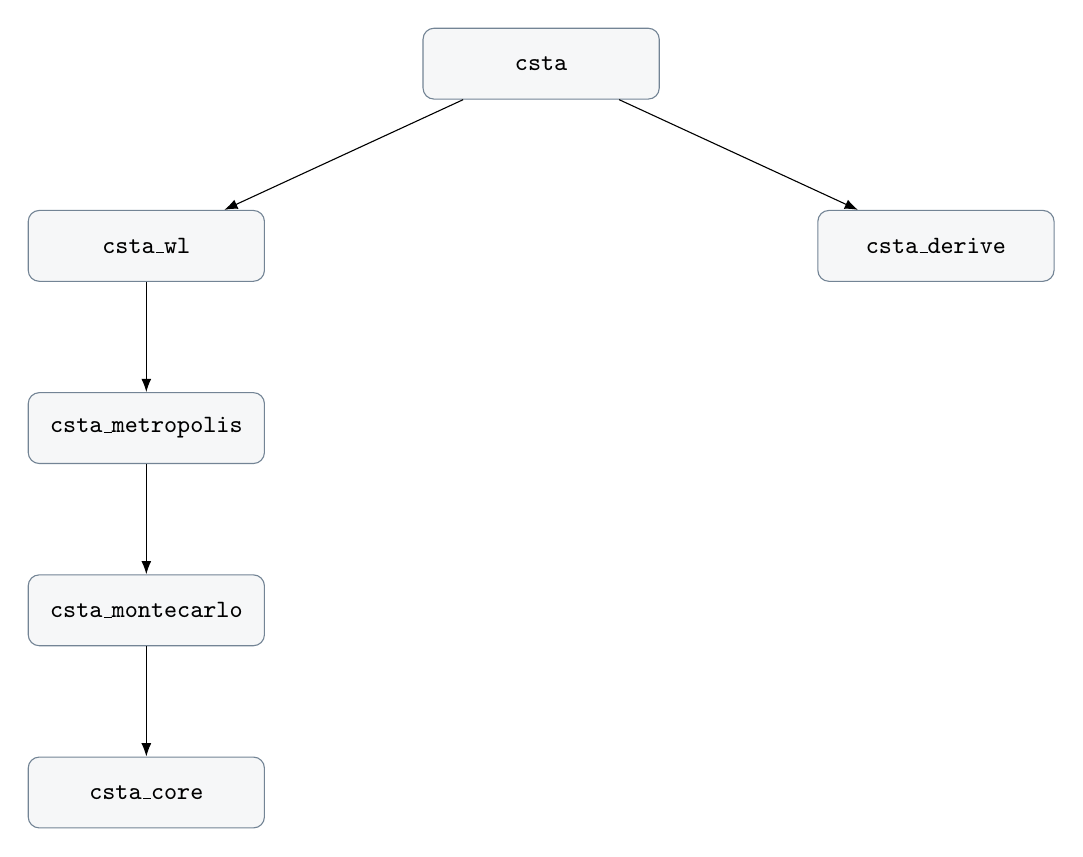
\begin{tikzpicture}[>=Latex,box/.style={draw=ink!60,rounded corners,
 fill=ink!4,minimum width=30mm,minimum height=9mm,font=\small\ttfamily},
 node distance=14mm and 20mm]
\node[box] (facade) {csta};
\node[box,below left=of facade] (wl) {csta\_wl};
\node[box,below right=of facade] (derive) {csta\_derive};
\node[box,below=of wl] (metro) {csta\_metropolis};
\node[box,below=of metro] (mc) {csta\_montecarlo};
\node[box,below=of mc] (core) {csta\_core};
\draw[->] (facade)--(wl);
\draw[->] (facade)--(derive);
\draw[->] (wl)--(metro);
\draw[->] (metro)--(mc);
\draw[->] (mc)--(core);
\end{tikzpicture}
\caption{Main dependency spine; arrows point to dependencies. Additional direct
edges let the facade re-export lower layers and let WL and Metropolis use core
utilities. The derive crate emits code that refers to the facade; it does not
introduce a runtime dependency cycle.}
\end{figure}

\section{Public entry points and dependencies}
\api{csta} re-exports vector types, canonical types, and random utilities.
Geometry and dynamics remain modules; Wang--Landau is \api{csta::wl}.
The prelude additionally imports observer traits. Explicit imports are helpful in
larger programs: a glob import includes the canonical \api{Result<T>} alias,
which has one type parameter. Use \api{std::result::Result<T, E>} when a different
error type is needed.

Direct use of an owning crate is supported. Runtime dependencies must continue
pointing from algorithms toward primitives; the lower crates do not depend on
\api{csta}. The procedural macro generates references to \api{csta} and
\api{rand}, so consumers of the derive need those dependency names available.

\par\noindent\begin{minipage}{\linewidth}
\begin{lstlisting}[caption={Dependency excerpt for a separate project. Adjust the local path.}]
[package]
name = "physics-experiment"
version = "0.1.0"
edition = "2024"
rust-version = "1.98.0"

[dependencies]
csta = { path = "../csta2/csta" }
rand = "=0.10.2"
\end{lstlisting}
\end{minipage}\par

Default features are empty. \api{serde} enables core serialization support.
\api{checkpoint} enables the sampler persistence stack and the serializable
PCG64 generator; it also enables the required Serde support. Ordinary runs do not
need either feature. Dependency versions and path relationships are fixed by the
workspace manifests and lockfile; toolchain requirements should not be reduced
to fit an older local compiler.
\src{Cargo.toml}
\src{csta/src/lib.rs}
\src{csta/src/prelude.rs}

\chapter{Physical and numerical conventions}\label{ch:conventions}
\section{Units and ensembles}
The APIs use bare floating-point numbers. They do not encode dimensions or
convert units. Choose a consistent energy scale, length scale, mass scale, and
time scale before constructing a model. The inverse temperature is always
\begin{equation}
  \beta=\frac{1}{k_B T}.
\end{equation}
Examples use reduced units with $k_B=1$. A canonical transition targets weights
proportional to $\exp(-\beta H)$. The lattice gas supplies $H-\mu N_p$ as its
\api{State::energy}; this produces a grand-canonical distribution over binary
site occupations. DOS sampling targets a distribution flattened in the supplied
energy bins. Dynamics advances a deterministic trajectory under a force law.

Finite negative $\beta$ is accepted by the generic canonical and DOS APIs.
Its physical use requires a normalizable spectrum, generally bounded above.
A truncated DOS always defines a finite supplied spectrum, even when the
untruncated physical system would not admit that ensemble. Wolff updates have a
more restrictive nonnegative-$\beta$ domain.

\begin{table}[htbp]
\small\centering
\begin{tabularx}{\textwidth}{@{}lY@{}}
\toprule
Quantity & Convention\\\midrule
\api{State::energy} & Total effective Hamiltonian; not energy per site.\\
$M$ & Signed total magnetization unless the caller deliberately defines another observable.\\
\api{ThermalSummary} & Energy, magnetization, heat capacity, and susceptibility
per site; Binder cumulant dimensionless.\\
\api{WLData::specific_heat} & Total $C=k_B\beta^2\Var(E)$; divide by size externally.\\
\api{dos()} & Natural logarithm of a degeneracy or continuous-bin mass.\\
Canonical step & One attempted proposal, including rejection or a self-loop.\\
Wolff step & One cluster update, whose number of flipped spins varies.\\
Dynamics step & One time increment $\Delta t$; unrelated to Monte Carlo time.\\
\bottomrule
\end{tabularx}
\caption{Conventions that must remain explicit in data analysis.}
\end{table}

\section{Floating-point range and errors}
Vectors have \api{f32} and \api{f64} variants; sampling energies and statistical
analysis use \api{f64}. Finite inputs do not ensure that every product, difference,
or sum is representable. Checked numerical APIs reject nonfinite results where
specified. Raw vector operators retain IEEE arithmetic, including infinities
and NaNs. There is no arbitrary-precision fallback.

Logarithmic weights avoid direct exponentiation of large energies or DOS values.
They reduce overflow risk, but do not make absolute partition functions or
moments representable in every scale. DOS updates smaller than floating-point
resolution are explicit errors. Changing units or removing an irrelevant DOS
offset can be necessary before starting a new run.

Most validation failures are returned as \api{Result}. Undefined statistical
estimates often use \api{Option} inside a successful result. These are different
outcomes: \api{None} can mean insufficient data, while \api{Err} means invalid
input or a failed numerical operation. Legacy sampling conveniences and
infallible random construction can panic. Error boundaries are summarized in
Chapter~\ref{ch:validation}.

\section{What a seed controls}
An explicit RNG makes randomness part of the simulation state. Repeating a seed
is meaningful only with the same algorithm, initial model, parameter values,
proposal ordering, dependency implementation, and relevant platform behavior.
Changing a callback, adding a random draw, or changing a chunk boundary can
change the trajectory. A seed alone is insufficient experiment metadata.

Record the Hamiltonian, boundary conditions, size, units, seed/RNG, schedules,
energy support, stopping reason, and software versions with results. Statistical
error bars should be accompanied by the number of observations, correlation or
block assumptions, and evidence from independent runs when available.

\chapter{Core vectors and geometry}\label{ch:core}
\section{Small floating vectors}
\api{Vec2f32}, \api{Vec2f64}, \api{Vec3f32}, \api{Vec3f64},
\api{Vec4f32}, and \api{Vec4f64} are public tuple structs. They provide
constructors, coordinate accessors, array/tuple conversions, precision
conversions, arithmetic, dot products, lengths, distances, and normalization.
They are \api{Copy}; optional Serde support serializes their coordinates.

Length uses chained hypotenuse calculations. Normalization first rescales by
the largest absolute coordinate, which allows a finite direction to be recovered
from many very large or very small vectors. \api{try_normalize} returns
\api{None} for zero vectors or nonfinite coordinates. \api{normalize} returns
the zero vector in those cases.

Squared length and dot products use direct arithmetic and can overflow even
when a normalized direction exists. Distance subtracts coordinates before
computing length; the subtraction itself can overflow. Narrowing from \api{f64}
to \api{f32} can lose precision or become infinite. Scalar division, including
\api{/=}, follows IEEE division. There are no checked arithmetic operators,
matrices, cross-product API, or dimensioned physical quantities.

\par\noindent\begin{minipage}{\linewidth}
% example: vectors
\begin{lstlisting}[language=Rust,caption={Vector arithmetic and explicit undefined directions.}]
use csta::{Vec2f64, Vec3f64};

fn main() {
    let v = Vec3f64::new(3.0, 4.0, 0.0);
    assert_eq!(v.len(), 5.0);
    assert!((v.try_normalize().unwrap().len() - 1.0).abs()
        < 1e-14);
    assert!(Vec2f64::default().try_normalize().is_none());
    let huge = Vec2f64::new(f64::MAX, f64::MAX);
    assert!(huge.len().is_infinite());
    assert!(huge.try_normalize().is_some());
}
\end{lstlisting}
\end{minipage}\par

\section{Periodic coordinates and nearest images}
\api{PeriodicBox<D>} represents an orthorhombic box with $D>0$ finite, positive
side lengths. \api{wrap} maps finite positions into $[0,L_d)$ for each coordinate.
\api{displacement(from, to)} returns the nearest-image displacement in
$[-L_d/2,L_d/2)$. Exact half-box ties choose the negative side. Both endpoints are
wrapped before subtraction, reducing overflow risk for large unwrapped positions.

The box does not store particles, apply forces, or impose a cutoff. It has no
triclinic cell matrix, shear convention, or long-range summation. The minimum
image is a geometric operation; the validity of a periodic interaction model is
a separate physical question.

\par\noindent\begin{minipage}{\linewidth}
% example: geometry
\begin{lstlisting}[language=Rust,caption={Periodic geometry and unique lattice bonds.}]
use csta::geometry::{Boundary, Lattice2D, PeriodicBox};

fn main() -> Result<(), Box<dyn std::error::Error>> {
    let cell = PeriodicBox::new([10.0, 8.0])?;
    assert_eq!(cell.wrap([-1.0, 9.0])?, [9.0, 1.0]);
    assert_eq!(cell.displacement([0.0; 2], [5.0, 0.0])?,
               [-5.0, 0.0]);
    let lattice = Lattice2D::new(3, 4, Boundary::Periodic)?;
    assert_eq!(lattice.len(), 12);
    assert_eq!(lattice.bonds().count(), 24);
    assert_eq!(lattice.neighbors(0)?.len(), 4);
    Ok(())
}
\end{lstlisting}
\end{minipage}\par

\section{Lattice topology}
\api{Lattice2D} stores a rectangular, row-major topology with open or periodic
boundaries. Open dimensions may be one; periodic dimensions must both be at least
three. This excludes ambiguous repeated-bond conventions on one- or two-site
periodic directions. Dimensions must be nonzero and their checked product must
fit the implementation's indexing range.

\api{neighbors(site)} returns up to four neighbors and rejects invalid indices.
\api{bonds()} emits each undirected nearest-neighbor pair once. This convention
sets the energy normalization used by the built-in two-dimensional models.
The topology supports neither arbitrary graphs nor three-dimensional lattices.
\src{csta_core/src/vec2.rs}
\src{csta_core/src/vec3.rs}
\src{csta_core/src/vec4.rs}
\src{csta_core/src/geometry.rs}

\chapter{Random construction}\label{ch:random}
\section{Trait and iterator}
\api{Randomizable::sample} constructs a value from a caller-provided RNG.
\api{MonteCarlo<T, R>} repeatedly calls it and is an infinite iterator. Use
\api{take}, an explicit loop bound, or another terminating consumer. Collecting
it without a bound does not terminate.

Built-in scalar \api{f32}/\api{f64} sampling is uniform on $[0,1)$. Built-in vector
coordinates are independent draws from that interval. This samples a cube, not
a sphere or a thermal velocity distribution. Tuple implementations cover arities
two through eight when each member implements the trait. General integer,
container, and constrained distributions are not supplied by a universal blanket
implementation.

\par\noindent\begin{minipage}{\linewidth}
% example: random
\begin{lstlisting}[language=Rust,caption={Bounded independent sampling and explicit physical distributions.}]
use csta::{MonteCarlo, gaussian, isotropic_direction};
use rand::{SeedableRng, rngs::StdRng};

fn main() -> Result<(), Box<dyn std::error::Error>> {
    let rng = StdRng::seed_from_u64(42);
    let values: Vec<f64> = MonteCarlo::new(rng).take(32).collect();
    assert!(values.iter().all(|x| (0.0..1.0).contains(x)));
    let mut rng = StdRng::seed_from_u64(43);
    let velocity = gaussian(&mut rng, 0.0, 1.0)?;
    let direction = isotropic_direction(&mut rng);
    assert!(velocity.is_finite());
    assert!((direction.len() - 1.0).abs() < 1e-14);
    Ok(())
}
\end{lstlisting}
\end{minipage}\par

\api{gaussian(rng, mean, scale)} uses Box--Muller sampling with finite mean and
finite nonnegative standard deviation. A zero scale returns the mean without
consuming randomness. Positive scale uses two draws; no companion Gaussian is
cached. A nonfinite result is an error. \api{isotropic_direction} uses uniform
$z\in[-1,1)$ and azimuth $\phi\in[0,2\pi)$ to return
$(\sqrt{1-z^2}\cos\phi,\sqrt{1-z^2}\sin\phi,z)$ on $S^2$.
Neither helper performs an ensemble equilibration step.

\section{Deriving random models}
The derive supports named, tuple, and unit structs, plus nonempty enums with
those variant shapes. Unconfigured fields use \api{Randomizable}. Generic bounds
are generated for sampled or defaulted field types as needed. Enum variants are
uniform unless every variant declares a weight.

\begin{longtable}{@{}P{0.34\textwidth}P{0.61\textwidth}@{}}
\toprule Attribute & Meaning and constraint\\\midrule\endhead
\api{range(a..b)} & Random range, excluding $b$; inclusive ranges use
\api{a..=b}. Invalid literal endpoints are compile errors. Dynamic invalid ranges
can panic at sampling time.\\
\api{len(n)} & Construct a \api{Vec} of sampled members. The length must convert
to \api{usize}; allocation remains the caller's responsibility.\\
\api{default} & Use the field type's \api{Default}.\\
\api{default = expr} & Evaluate an explicit initializer, including dependencies
on other named fields.\\
\api{after(expr)} & Sample the field first, then evaluate its transformation.\\
\api{mul}, \api{div}, \api{add}, \api{sub} & Arithmetic transforms in attribute
order; do not combine with a conflicting base initializer.\\
\api{weight = literal} & Enum variant weight. All variants must declare finite,
nonnegative numeric weights, with at least one positive value.\\
\bottomrule
\end{longtable}

\par\noindent\begin{minipage}{\linewidth}
% example: derive
\begin{lstlisting}[language=Rust,caption={A bounded proposal type constructed by the derive macro.}]
use csta::{Randomizable, csta_derive};
use rand::{SeedableRng, rngs::StdRng};

#[derive(csta_derive::Randomizable)]
struct Proposal {
    #[csta(range(-0.5..0.5))]
    displacement: f64,
    #[csta(default = displacement * displacement)]
    squared: f64,
    #[csta(len(3))]
    auxiliary: Vec<f64>,
}

fn main() {
    let p = Proposal::sample(&mut StdRng::seed_from_u64(42));
    assert!((-0.5..0.5).contains(&p.displacement));
    assert_eq!(p.squared, p.displacement * p.displacement);
    assert_eq!(p.auxiliary.len(), 3);
}
\end{lstlisting}
\end{minipage}\par

Named-field dependencies are analyzed syntactically and evaluated in dependency
order. Cycles, unknown attributes, conflicting initializers, empty enums, and
unions produce compiler diagnostics. Avoid shadowing field names inside
initializer expressions: the dependency analysis does not perform full Rust name
resolution. Attribute expressions can use \api{rng}.

Weights are rescaled by their maximum to avoid an overflowing total. Zero-weight
variants are never selected. Extreme weight ratios can still lose representable
probability. The derive is an infallible constructor, not a general distribution
language or a proof that sampled states satisfy a Hamiltonian's constraints.
\src{csta_montecarlo/src/lib.rs}
\src{csta_derive/src/lib.rs}
\src{csta_derive/README.md}

\chapter{The model contract}\label{ch:state}
\section{State, parameters, and reversible changes}
\api{State} separates physical configuration from Hamiltonian parameters and
proposal descriptions. Both canonical and Wang--Landau sampling use it. A
\api{Change} must be cloneable; parameters used by checked execution must provide
an independent \api{Clone}. The minimum interface is:

\par\noindent\begin{minipage}{\linewidth}
\begin{lstlisting}[language=Rust,caption={Required trait methods; interface excerpt.}]
trait State {
    type Params;
    type Change: Clone;
    fn energy(&self, params: &mut Self::Params) -> f64;
    fn propose_change(&self, rng: &mut impl rand::RngExt)
        -> Self::Change;
    fn apply_change(&mut self, change: Self::Change);
    fn revert_change(&mut self, change: Self::Change);
}
\end{lstlisting}
\end{minipage}\par

\api{energy} may refresh a parameter cache. Rejected moves restore the parameter
snapshot. A clone that shares mutable cache storage through interior mutability
cannot provide that guarantee. A cache held inside the state must be restored by
\api{revert_change} itself. Store the previous cached value in \api{Change} when
inverse floating-point arithmetic would not restore it exactly.

Parameters describe a fixed Hamiltonian during a sampling run. Mutating physical
parameters through an energy cache changes the target distribution and violates
the contract. All model methods must terminate. Cancellation is cooperative and
cannot preempt a callback that loops indefinitely.

\section{Optional hooks}
\api{log_proposal_ratio(&self, &change)} returns
\begin{equation}
 c(x,y)=\log\frac{q(x\mid y)}{q(y\mid x)}.
\end{equation}
It is evaluated before applying the move and defaults to zero, which assumes
symmetric proposals. Negative infinity means zero reverse probability and rejects
the move. NaN and positive infinity are invalid. \api{Hastings<S,F>} supplies the
same correction through a closure without changing the wrapped model type's
implementation.

\par\noindent\begin{minipage}{\linewidth}
% example: hastings
\begin{lstlisting}[language=Rust,caption={Correcting an asymmetric independence proposal.}]
use csta::{Hastings, Metropolis, State};
use rand::{RngExt, SeedableRng, rngs::StdRng};

struct Bit(bool);
impl State for Bit {
    type Params = ();
    type Change = (bool, bool);
    fn energy(&self, _: &mut ()) -> f64 { f64::from(self.0) }
    fn propose_change(&self, rng: &mut impl RngExt) -> Self::Change {
        (self.0, rng.random_bool(0.75))
    }
    fn apply_change(&mut self, (_, next): Self::Change) {
        self.0 = next;
    }
    fn revert_change(&mut self, (old, _): Self::Change) {
        self.0 = old;
    }
}

fn main() -> Result<(), Box<dyn std::error::Error>> {
    let model = Hastings {
        state: Bit(false),
        log_ratio: |_: &Bit, &(old, next): &(bool, bool)| {
            let q = |b| if b { 0.75_f64 } else { 0.25 };
            (q(old) / q(next)).ln()
        },
    };
    let mut run = Metropolis::with_all(
        model, (), 1.0, 2_000, StdRng::seed_from_u64(42),
    );
    assert_eq!(run.run(None)?.attempted, 2_000);
    Ok(())
}
\end{lstlisting}
\end{minipage}\par

Here the proposal draws the next bit independently with probability 0.75 for
true. Its reverse/forward ratio is $q(\text{old})/q(\text{next})$. Including that
factor targets the canonical excited probability $1/(1+e^\beta)$; using zero
correction would retain the proposal's bias. A self-loop has correction zero.

\api{delta_energy} optionally returns a local $H(y)-H(x)$; \api{None} requests
full energy evaluation. Only use it when accepted moves do not require a skipped
parameter-cache refresh. \api{valid_state} defaults to true and is used in
checkpoint validation; custom persisted models should override it to check
structural invariants. It is not an automatic per-proposal physical validator.

\par\noindent\begin{minipage}{\linewidth}
% example: custom_state
\begin{lstlisting}[language=Rust,caption={A complete reversible two-level model.}]
use csta::{Metropolis, State};
use rand::{RngExt, SeedableRng, rngs::StdRng};

#[derive(Clone)]
struct TwoLevel { excited: bool }

impl State for TwoLevel {
    type Params = f64; // excitation gap
    type Change = bool; // previous state
    fn energy(&self, gap: &mut f64) -> f64 {
        if self.excited { *gap } else { 0.0 }
    }
    fn propose_change(&self, _: &mut impl RngExt) -> bool {
        self.excited
    }
    fn apply_change(&mut self, old: bool) {
        self.excited = !old;
    }
    fn revert_change(&mut self, old: bool) {
        self.excited = old;
    }
}

fn main() -> Result<(), Box<dyn std::error::Error>> {
    let mut run = Metropolis::with_all(
        TwoLevel { excited: false }, 1.0, 0.7, 2_000,
        StdRng::seed_from_u64(42),
    );
    let report = run.run(None)?;
    assert_eq!(report.attempted, 2_000);
    Ok(())
}
\end{lstlisting}
\end{minipage}\par

This deterministic toggle proposal is symmetric. At $\beta=0$ it alternates
between states and is periodic; a self-loop proposal would be needed to remove
that periodicity. At the positive $\beta$ shown, energetic rejections provide
self-loops. Generic trait conformance does not establish irreducibility,
aperiodicity, or adequate exploration.
\src{csta_metropolis/src/lib.rs}

\chapter{Canonical sampling and observations}\label{ch:canonical}
\section{Transition and rollback}
A canonical proposal uses the log acceptance ratio
\begin{equation}
 r=\beta\bigl[H(x)-H(y)\bigr]+c(x,y),\qquad
 \alpha(x,y)=\min(1,e^r).
\end{equation}
The implementation compares $\log u$ with $r$ and avoids exponentiating it.
Finite energy and finite $\beta$ are required. Overflow of a valid Boltzmann log
ratio has its limiting acceptance meaning; an indeterminate ratio is an error.
At $\beta=0$, the Boltzmann part is zero before any potentially overflowing energy
subtraction.

\api{try_step} validates counters, snapshots parameters, evaluates old energy,
constructs a proposal and correction, applies it, evaluates the proposed energy,
and accepts or restores the move. On a checked proposal error, the state,
parameters, and attempt counts are restored under the model contract. Random
draws already consumed are not rewound. Panics in user model methods are not a
checked transactional error path.

A completed rejection still increments \api{attempted_moves}. Accepted self-loops
count as accepted moves. Lifetime acceptance is accepted divided by attempted;
both accepted and rejected rates are zero before any attempts. Public fields
allow explicit control, but callers can also invalidate a model, cache, or
counter by mutating them directly.

\section{Budgets and observation timing}
\api{with_all(state, params, beta, steps, rng)} is the most explicit constructor.
Convenience constructors fill defaults or use the thread RNG. Constructor names
ending in \api{no_beta} use $\beta=1$. Construction itself is not a checked run;
execution performs validation.

\api{run} executes at most \api{steps} proposals per call and returns a
\api{RunReport} with this call's attempts, accepts, and \api{Complete} or
\api{Cancelled}. Lifetime counters accumulate across calls. \api{try_step}
returns one checked acceptance decision. Legacy \api{step}, \api{run_empty}, and
observer conveniences panic on invalid execution instead of returning errors.

A \api{Schedule} skips \api{burn_in} completed proposals and then measures every
\api{stride} proposals. The first measurement is at
$\text{burn\_in}+\text{stride}$. Stride must be positive, and schedules restart
for each run call. Measurements describe the retained state after the move,
including repeated states after rejection. Counting accepted states alone would
change the sampled measure.

\par\noindent\begin{minipage}{\linewidth}
% example: canonical
\begin{lstlisting}[language=Rust,caption={Streaming canonical observations with constant-memory blocking.}]
use csta::{Metropolis, Schedule, models::Ising2D};
use csta::statistics::Blocking;
use rand::{SeedableRng, rngs::StdRng};

fn main() -> Result<(), Box<dyn std::error::Error>> {
    let mut run = Metropolis::with_all(
        Ising2D::aligned(4)?, (), 0.4, 12_000,
        StdRng::seed_from_u64(42),
    );
    let mut energy = Blocking::new(128)?;
    let report = run.try_run_observed(
        Schedule { burn_in: 2_000, stride: 1 }, None,
        |s, _| energy.push(s.recompute_energy() / 16.0),
    )?;
    assert_eq!(report.attempted, 12_000);
    assert_eq!(energy.moments().count(), 10_000);
    println!("energy/site estimate: {:?}", energy.estimate());
    Ok(())
}
\end{lstlisting}
\end{minipage}\par

\section{Observer interfaces}
\api{run_observed} accepts an infallible streaming closure;
\api{try_run_observed} accepts a closure returning the canonical \api{Result<()>}.
A measurement error occurs after a committed move and leaves the run at that
move. External output and callback side effects are not rolled back.

\api{Observer} provides static measurement, interval, and finalization methods.
\api{DynObserver} provides the corresponding instance-based interface.
\api{run_with} returns one collected series; \api{run_with_2},
\api{run_with_3}, and \api{run_with_4} collect heterogeneous observer outputs.
\api{run_with_n} handles dynamic observers with a common output type. These
interfaces retain observations in memory; a streaming closure can maintain only
moments, blocks, or a file sink.

Burn-in and thinning are controls, not automatic equilibration detection.
Acceptance rate does not measure mixing by itself. Observing every proposal is
often useful for estimating temporal dependence; changing stride changes the time
unit of the resulting autocorrelation estimate.
\src{csta_metropolis/src/lib.rs}
\src{csta_metropolis/src/observer.rs}

\chapter{Lattice models and temperature exchange}\label{ch:models}
\section{Two-dimensional Ising model}
\api{models::Ising2D} uses rectangular \api{Lattice2D} connectivity and spins
$s_i\in\{-1,+1\}$:
\begin{equation}
 H=-J\sum_{\langle ij\rangle}s_i s_j-h\sum_i s_i,
 \qquad M=\sum_i s_i.
\end{equation}
Each bond appears once. Construction validates finite $J,h$, spin values, lattice
size, and boundary rules. \api{aligned(L)} is the periodic $L\times L$ model with
all spins positive, $J=1$, and $h=0$.

A single-site flip has
$\Delta H=2s_i(J\sum_{j\sim i}s_j+h)$. The model caches total energy and records
the previous cached value in each change for exact rejection rollback.
\api{recompute_energy} provides an independent full traversal; magnetization
also traverses the lattice. Repeated accepted floating-point updates can drift
relative to recomputation, so noninteger couplings warrant periodic comparisons
in a validation study.

\api{wolff_step(beta, rng)} is restricted to $J\geq0$, $\beta\geq0$, and $h=0$.
It grows a cluster through aligned neighbors with
$p=1-\exp(-2\beta J)$ and flips that cluster, following the usual ferromagnetic
construction~\cite{janke}. It returns cluster size. At $\beta J=0$, the cluster is
a single spin. The implementation uses lattice-sized scratch storage and
recomputes total energy after the update; total work is therefore $O(N_s)$ even
when the cluster is small. It has no general field or frustrated-spin extension.

\section{Lattice gas}
\api{models::LatticeGas} stores binary occupations $n_i\in\{0,1\}$ on the same
topology. Its physical interaction energy is $H=-J\sum_{\langle ij\rangle}n_i n_j$;
\api{State::energy} returns $H-\mu N_p$ with $N_p=\sum_i n_i$.
A uniformly chosen site is toggled, so insertion and removal proposals are
symmetric on this configuration space. There are no continuum volume,
factorial, or particle-selection corrections to add for this specific move.

\api{physical_energy} excludes the chemical potential. Use it when reporting
$H$, and use the effective energy for acceptance or reweighting at fixed $\mu$.
The model has cached reversible energy updates. It does not implement mobile
particles, continuum insertions, or a general grand-canonical acceptance helper.

\par\noindent\begin{minipage}{\linewidth}
% example: lattice_models
\begin{lstlisting}[language=Rust,caption={Cluster updates and a grand-canonical lattice gas.}]
use csta::{Metropolis, State, models::{Ising2D, LatticeGas}};
use csta::geometry::Boundary;
use rand::{SeedableRng, rngs::StdRng};
fn main() -> Result<(), Box<dyn std::error::Error>> {
    let mut rng = StdRng::seed_from_u64(42);
    let mut spins = Ising2D::aligned(4)?;
    let cluster = spins.wolff_step(0.4, &mut rng)?;
    assert!((1..=16).contains(&cluster));
    let gas = LatticeGas::new(4, 4, Boundary::Periodic,
                             1.0, -2.0, vec![false; 16])?;
    let mut run = Metropolis::with_all(gas, (), 0.5, 1_000, rng);
    run.run(None)?;
    println!("effective energy: {}", run.state.energy(&mut ()));
    println!("physical energy: {}", run.state.physical_energy());
    Ok(())
}
\end{lstlisting}
\end{minipage}\par

\section{Temperature replica exchange}
\api{replica::ReplicaExchange} accepts one initial state per finite, strictly
increasing inverse temperature, a common parameter value, and a seed. Parameters
are independently cloned. Local Metropolis chunks run sequentially; adjacent
pairs alternate between two disjoint pairing patterns.

For temperatures $\beta_i,\beta_j$ and energies $E_i,E_j$, the swap log ratio is
\begin{equation}
 r_{\rm swap}=(\beta_i-\beta_j)(E_i-E_j).
\end{equation}
Configurations, parameter caches, and identity labels move between slots.
Temperatures, local RNGs, and local move counters remain attached to the slots.
The common-Hamiltonian assumption is essential; this is not general Hamiltonian
replica exchange.

\par\noindent\begin{minipage}{\linewidth}
% example: temperature_replicas
\begin{lstlisting}[language=Rust,caption={An explicit inverse-temperature ladder.}]
use csta::{models::Ising2D, replica::ReplicaExchange};
fn main() -> Result<(), Box<dyn std::error::Error>> {
    let states = vec![Ising2D::aligned(4)?; 3];
    let mut replicas = ReplicaExchange::new(states, (),
                                          vec![0.2, 0.4, 0.6], 42)?;
    replicas.run(20, 100, None)?; // rounds, local proposals
    println!("swaps: {}/{}", replicas.swap_accepts,
             replicas.swap_attempts);
    println!("round trips: {}", replicas.round_trips);
    Ok(())
}
\end{lstlisting}
\end{minipage}\par

Swap attempts, accepts, and cold--hot--cold round trips are separate diagnostics.
A single replica is valid and performs no exchange. A saved local cursor allows
cancellation in a chunk to resume using the original \api{local_steps}; the
requested round count includes completion of a pending round. A whole round is
not an atomic transaction. Direct \api{exchange(i)} calls do not perform the
round-trip bookkeeping that the round runner performs.

The ladder is explicit; no automatic optimization or CPU-parallel execution is
provided. Poor energy overlap suppresses swaps. Good swap acceptance alone does
not establish barrier crossing.
\src{csta_metropolis/src/models.rs}
\src{csta_metropolis/src/replica.rs}

\chapter{Statistics and finite-size analysis}\label{ch:statistics}
\section{Streaming moments}
\api{Moments} stores count, mean, and centered second-moment sum. Welford-style
updates and Chan-style merges avoid direct subtraction of large raw second
moments. \api{variance} uses $n-1$ and needs at least two samples;
\api{population_variance} uses $n$ and needs one. Empty means are \api{None}.
Nonfinite observations, numerical overflow, and counter overflow are errors;
failed updates leave the previous accumulator intact.

\api{Covariance} similarly accumulates paired scalar observations and returns
sample covariance for $n>1$. These accumulators estimate moments, not independent
sample counts. Correlated observations require an additional error estimator.

\section{Blocking and autocorrelation}
\api{Blocking} uses nonoverlapping fixed-size blocks and constant memory. It
requires at least eight complete blocks and positive block-mean variance before
returning an estimate. The standard error is
\begin{equation}
 \SE(\bar A)=\sqrt{\frac{s^2_{\rm block\ means}}{B}},
 \qquad
 \ESS=\min\left(\frac{s^2_{\rm completed\ observations}}
                         {\SE(\bar A)^2},\,Bb\right),
\end{equation}
where $b$ is block length and $B$ is the number of complete blocks. An incomplete
trailing block is excluded from the estimate's mean, uncertainty, and sample
count. \api{moments()} still includes every observation. The default block length
is 64; no automatic choice or decorrelation guarantee is implied.

\api{correlated_estimate} analyzes an explicitly retained scalar series. It uses
positive adjacent autocovariance pairs with a nonincreasing constraint, in the
initial-sequence family~\cite{geyer}. With lag autocorrelation $\rho_k$, its
convention is $\tau=1+2\sum_{k>0}\rho_k$, so
$\ESS=n/\tau$ and $\SE^2\approx\gamma_0\tau/n$. This $\tau$ is twice the
integrated time under the alternative $\tfrac12+\sum\rho_k$ convention.

The implementation floors $\tau$ at one. It requires at least 32 nonconstant
observations, a resolved nonpositive pair before the lag cap, and $n\geq20\tau$.
The cap is $\min(n/2,4096)$; unresolved series return \api{None}. Work is
$O(n\min(n/2,4096))$. Its assumptions concern stationary reversible chains.
It does not diagnose equilibration, and should not be applied uncritically to
adaptive WL output or arbitrary deterministic dynamics.

\section{Thermodynamic summaries and nonlinear errors}
\api{Thermodynamics::push(E,M)} consumes total energy and signed total
magnetization. With $N_s$ sites, \api{summary(beta,k_b,sites)} computes
\begin{align}
 e &= \mean{E}/N_s, & m &= \mean{M}/N_s,\\
 c &= k_B\beta^2\Var(E)/N_s, & \chi &= \beta\Var(M)/N_s,\\
 U_4 &= 1-\frac{\mean{M^4}}{3\mean{M^2}^2}. &&
\end{align}
The variances in these fluctuation formulas use population moments. The Binder
cumulant is \api{None} when its denominator vanishes. The API requires finite
$\beta$, positive finite $k_B$, nonzero site count, and at least one observation.
It does not replace $M$ with $|M|$ or infer a symmetry-breaking convention.

\api{thermal_errors} applies a delete-one-block jackknife to these nonlinear
summaries. It needs at least eight complete blocks, accepts at most 4096 blocks,
and discards trailing incomplete samples. Combining leave-one-block summaries
costs $O(B^2)$ after reading the observations. Constant complete data can return
\api{None}; blocks must be chosen longer than the relevant correlation scale.
The summary alone provides no uncertainty estimate.

\par\noindent\begin{minipage}{\linewidth}
% example: thermal_statistics
\begin{lstlisting}[language=Rust,caption={Thermodynamic summaries with an explicit size and block length.}]
use csta::{State, models::Ising2D};
use csta::statistics::{Thermodynamics, thermal_errors};
use rand::{SeedableRng, rngs::StdRng};

fn main() -> Result<(), Box<dyn std::error::Error>> {
    let mut model = Ising2D::aligned(4)?;
    let mut rng = StdRng::seed_from_u64(42);
    let mut moments = Thermodynamics::default();
    let mut pairs = Vec::new();
    for i in 0..5_000 {
        model.wolff_step(0.4, &mut rng)?;
        if i >= 1_000 {
            let pair = (model.energy(&mut ()), model.magnetization());
            moments.push(pair.0, pair.1)?;
            pairs.push(pair);
        }
    }
    println!("{:?}", moments.summary(0.4, 1.0, 16)?);
    println!("{:?}", thermal_errors(&pairs, 0.4, 1.0, 16, 128)?);
    Ok(())
}
\end{lstlisting}
\end{minipage}\par

\section{Finite-size helpers}
\api{finite_size::crossings} linearly interpolates every crossing of two curves
on an exactly shared, finite, strictly increasing coordinate grid. Empty and
multiple results remain explicit; a coincident segment is ambiguous and returns
an error. \api{peak} returns a unique observed interior maximum, or \api{None}
for a tie or boundary maximum. Neither routine fits a scaling law or extrapolates.

\api{block_bootstrap} resamples complete nonoverlapping blocks with replacement
and evaluates a user-supplied scalar statistic. It returns the bootstrap standard
deviation. It requires a positive block size, at least eight blocks, at least two
repetitions, and finite data; incomplete trailing samples are excluded. Choosing
a block length and a physically appropriate statistic remains the caller's task.

\par\noindent\begin{minipage}{\linewidth}
% example: finite_size
\begin{lstlisting}[language=Rust,caption={Explicit crossings and peaks on a finite grid.}]
use csta::finite_size::{crossings, peak};

fn main() -> Result<(), Box<dyn std::error::Error>> {
    let a = [(0.0, 0.0), (1.0, 1.0), (2.0, 0.0)];
    let b = [(0.0, 0.5), (1.0, 0.5), (2.0, 0.5)];
    assert_eq!(crossings(&a, &b)?, vec![0.5, 1.5]);
    assert_eq!(peak(&a)?, Some((1.0, 1.0)));
    assert!(peak(&b)?.is_none());
    Ok(())
}
\end{lstlisting}
\end{minipage}\par

For a finite-size study, collect independent or appropriately blocked curves for
several sizes, retain all crossings, and vary the temperature grid and block
length. A finite-size susceptibility peak or Binder crossing is not itself a
thermodynamic-limit critical point. These helpers provide neither critical
exponents nor automated model selection, fit covariance, or plotting.
\src{csta_metropolis/src/statistics.rs}
\src{csta_metropolis/src/finite_size.rs}

\chapter{Deterministic dynamics}\label{ch:dynamics}
\section{A separate NVE interface}
\api{dynamics::Dynamics<D>} stores vectors of positions, velocities, and positive
masses. $D$ must be positive, particle arrays must be nonempty and equally sized,
and all coordinates and velocities must be finite. The API uses arrays
\api{[f64; D]} rather than the small-vector types. It does not require
\api{State}, an RNG, or a Monte Carlo acceptance rule.

A force callback maps positions to a potential energy and one force vector per
particle. Forces must be consistent with the potential and be pure functions of
the supplied coordinates. Fixed-step velocity-Verlet~\cite{lammps} advances
\begin{align}
 \mathbf v_{i,n+1/2}&=\mathbf v_{i,n}
     +\frac{\Delta t}{2m_i}\mathbf F_i(\mathbf r_n),\\
 \mathbf r_{i,n+1}&=\mathbf r_{i,n}
     +\Delta t\,\mathbf v_{i,n+1/2},\\
 \mathbf v_{i,n+1}&=\mathbf v_{i,n+1/2}
     +\frac{\Delta t}{2m_i}\mathbf F_i(\mathbf r_{n+1}).
\end{align}
The step size must be finite and positive. Two force evaluations and a cloned
candidate particle state are used per step; forces are not cached between calls.
A failed step leaves the original particles unchanged, but cannot undo external
callback effects. A failed multi-step run retains earlier successful steps.

\section{Energy monitoring and force helpers}
\api{run} returns initial energy, final energy, and maximum absolute drift from
the initial value. Absolute drift avoids division by zero. Zero steps are valid
with a valid time step and initial energy. A finite trajectory can still be
unstable or inaccurate; users must compare time steps and impose a suitable
drift tolerance. An NVE trajectory is not automatically an ergodic sample of an
energy surface.

\par\noindent\begin{minipage}{\linewidth}
% example: dynamics
\begin{lstlisting}[language=Rust,caption={A harmonic trajectory with an explicit drift check.}]
use csta::dynamics::{Dynamics, harmonic};

fn main() -> Result<(), Box<dyn std::error::Error>> {
    let mut particles = Dynamics::new(
        vec![[1.0]], vec![[0.0]], vec![1.0],
    )?;
    let drift = particles.run(1_000, 0.001, |x| harmonic(x, 1.0))?;
    assert!(drift.maximum_absolute < 1e-6);
    assert!((particles.positions()[0][0] - 1.0_f64.cos()).abs()
        < 1e-6);
    Ok(())
}
\end{lstlisting}
\end{minipage}\par

\api{harmonic} implements $U=\tfrac12 k\sum_i|\mathbf r_i|^2$ with finite
$k\geq0$. \api{lennard_jones} evaluates all nearest-image pairs in a supplied
orthorhombic box using
\begin{equation}
 U=4\epsilon\sum_{i<j}
 \left[\left(\frac{\sigma}{r_{ij}}\right)^{12}
       -\left(\frac{\sigma}{r_{ij}}\right)^6\right].
\end{equation}
It requires positive finite $\epsilon,\sigma$ and rejects coincident or
unrepresentable pair separations. Pair forces are equal and opposite. Positions
remain unwrapped in storage; the force helper applies nearest images.

The Lennard--Jones helper is a tiny-system example with $O(N_p^2D)$ work. It has
no cutoff, neighbor list, tail correction, electrostatics, or full periodic-image
sum. Minimum-image branch changes also require care for smooth dynamics. No
thermostat, barostat, constraints, adaptive time step, particle checkpoint API,
or production bulk-fluid accuracy claim is provided.
\src{csta_core/src/dynamics.rs}

\chapter{Energy grids and DOS data}\label{ch:grids}
\section{Explicit support}
\api{EnergyGrid::discrete(levels)} requires a nonempty sequence of finite,
strictly increasing energies with representable adjacent differences. Lookup is
exact. A single level is valid. Integer-valued energies represented exactly in
\api{f64} are convenient; a numerically rounded Hamiltonian must not rely on a
nearby level being accepted.

\api{EnergyGrid::continuous(min,max,bins)} requires finite $\min<\max$, positive
bin count, finite positive width, and distinct representable edges. Intervals
are half-open, except that the last includes the upper endpoint. Thermodynamic
calculations use stored bin centers. Finite energies outside the interval return
\api{None}; NaN and infinities return an error. The implementation does not clamp
energies into endpoint bins.

\par\noindent\begin{minipage}{\linewidth}
% example: grids
\begin{lstlisting}[language=Rust,caption={Endpoint behavior and an explicit inaccessible bin.}]
use csta::wl::{EnergyGrid, RawWangLandauData};

fn main() -> Result<(), Box<dyn std::error::Error>> {
    let continuous = EnergyGrid::continuous(-1.0, 1.0, 4)?;
    assert_eq!(continuous.bin(-1.0)?, Some(0));
    assert_eq!(continuous.bin(1.0)?, Some(3));
    assert_eq!(continuous.bin(1.01)?, None);
    assert!(continuous.bin(f64::NAN).is_err());
    let grid = EnergyGrid::discrete(vec![-2.0, 0.0, 2.0])?;
    let data = RawWangLandauData::with_support(
        grid, vec![true, false, true],
        vec![0.0, f64::NEG_INFINITY, 0.0],
    )?;
    assert_eq!(data.energy_to_bin(0.0)?, None);
    assert!(!data.is_flat());
    Ok(())
}
\end{lstlisting}
\end{minipage}\par

On an existing grid, \api{on_grid} initially gives every bin zero log-DOS.
The explicit constructor \api{with_support} takes a grid, mask, and log masses:
accessible entries must be finite, inaccessible entries must be negative
infinity, and at least one entry must be accessible. All arrays must match the
grid. The sampler never infers inaccessible states from missing visits.

A support mask can disconnect proposal paths. Declaring both endpoints of a path
accessible does not create a proposal connecting them. Conversely, an omitted
physical energy changes the ensemble being estimated. Support design therefore
requires model knowledge, not histogram inspection alone.

\section{Mass, density, and normalization}
DOS arrays contain $\ell_i=\ln g_i$. For a discrete level, $g_i$ is a state
count or degeneracy. For a continuous interval $I_i$, the intended quantity is
bin mass, $g_i=\int_{I_i}g(E)\,dE$. The partition sum uses $g_i$ directly; an
additional bin-width factor would count the width twice.

Sampling determines relative log-DOS values, leaving an additive constant
undetermined. \api{normalize_log_count(ln_total)} sets the log of total mass;
\api{anchor(i,ln_degeneracy)} sets one finite bin. Relative probabilities are
unchanged. Absolute free energy and entropy require a physically meaningful
normalization. A continuous model also needs a measure convention; the library
does not supply a phase-space cell, indistinguishability factor, or quantum scale.

Continuous-bin quadrature replaces energy within a bin by its center and assumes
constant DOS for acceptance within that bin. Binning error remains even after
arbitrarily long sampling. Vary bin width and support bounds separately from the
sampling budget. There is no automatic binning, adaptive grid, or interpolation
inside a bin.

\section{Data lifecycle and counters}
Raw data holds log-DOS, current-stage histogram, lifetime histogram, support,
and their visit totals. Fields are private and constructors validate shape.
\api{clear_hist} clears current counts only. \api{process_data} consumes raw
data into \api{WLData}, retaining the grid, log-DOS, and current histogram;
it does not retain all raw lifetime diagnostics.

A processed \api{WLData} can also be constructed from exact or externally
estimated data. Its histogram is bookkeeping and is not used as an alternative
DOS in thermodynamic calculations. Negative-infinite log masses represent absent
levels; at least one mass must be finite. Reusing an old DOS with fresh counters
starts a new adaptive experiment. It is not exact continuation of a previous
sampler.
\src{csta_wl/src/grid.rs}
\src{csta_wl/src/lib.rs}
\src{csta_wl/src/wl_data.rs}

\chapter{Serial Wang--Landau and SAMC}\label{ch:wl}
\section{Algorithm composition}
The implementation combines Wang--Landau preliminary stages with SAMC production.
The production schedule follows the trial-move convention described by
Shakirov~\cite{shakirov}. For a current bin $i$ and proposed accessible bin $j$,
the log acceptance ratio is
\begin{equation}
 r=\ell_i-\ell_j+c(x,y).
\end{equation}
A finite off-support proposal is rejected and the current state is retained.
A nonfinite energy is an error with rollback. After every completed proposal,
the retained bin $b$ receives
\begin{equation}
 \ell_b\gets\ell_b+\gamma,\qquad h_b\gets h_b+1.
\end{equation}
This update also occurs after rejection or a self-loop. The acceptance decision
uses the pre-update DOS. A positive update that overflows or rounds back to the
old value is rejected as a numerical operation; no visit is then recorded.

\section{Preliminary refinement}
A preliminary stage uses a constant update, initially \api{initial_ln_f}. With
$B_a$ accessible bins, a stage completes only after
\begin{equation}
 n_{\rm stage}\geq\max(\text{min\_stage\_steps},
                       B_a\,\text{visits\_per\_bin})
 \quad\text{and}\quad
 h_i\geq p\bar h\ \text{for every accessible }i.
\end{equation}
The mean $\bar h$ excludes masked bins and must be positive. Equality satisfies
the flatness threshold. \api{visits_per_bin} sets a minimum total stage budget;
it does not by itself require that number in every individual bin.

After a stage completes, the update is halved and the current histogram is
cleared. State, log-DOS, lifetime visits, and RNG continue. After the requested
number of stages, production starts with its own trial counter at zero.
Zero preliminary stages explicitly skips this phase.

\section{Production schedule and bounded execution}
Production uses
\begin{equation}\label{eq:samc}
 \gamma(t)=\frac{t_0}{t_1+t},
\end{equation}
where $t$ is the number of completed production trial moves before the current
proposal. Rejections count. It is not visits divided by bin count, physical time,
or number of accepted moves. Defaults are $t_0=B_a$ and $t_1=10t_0$.

\begin{longtable}{@{}P{0.28\textwidth}P{0.17\textwidth}P{0.49\textwidth}@{}}
\toprule Configuration field & Default & Range and meaning\\\midrule\endhead
\api{preliminary_stages} & 5 & 0--1024; final preliminary update must remain positive and representable.\\
\api{min_stage_steps} & 1000 & Positive \api{u64}; lower bound per stage.\\
\api{visits_per_bin} & 500 & Positive \api{u64}; product with accessible bins must not overflow.\\
\api{flatness} & 0.8 & Finite fraction in $(0,1]$.\\
\api{initial_ln_f} & 1.0 & Finite positive preliminary log-DOS increment.\\
\api{sampling_steps} & 100000 & Production trial target; zero performs no moves, including no warm-up.\\
\api{max_steps} & 10000000 & Positive total preliminary-plus-production bound.\\
\api{t0}, \api{t1} & Derived & Optional finite positive scales with representable positive updates over the requested schedule.\\
\bottomrule
\end{longtable}

\api{run} validates the grid, raw-data state, configuration, and initial energy.
The initial state must already lie inside accessible support. It requires
\api{State} and independent parameter cloning, but not \api{Randomizable}.
\api{sample_in_support} is an optional bounded initializer for models that also
implement \api{Randomizable}; attempts must be positive. Failure to find a state
returns \api{InitialStateOutside}. It is unsuitable as an unbounded search for a
rare window.

\par\noindent\begin{minipage}{\linewidth}
% example: serial_wl
\begin{lstlisting}[language=Rust,caption={A bounded serial DOS run with an explicit completion check.}]
use csta::wl::{self, Config, RawWangLandauData, models::Ising};
use rand::{SeedableRng, rngs::StdRng};

fn main() -> Result<(), Box<dyn std::error::Error>> {
    let result = wl::run(
        Ising::<4>::new([1; 4])?, (),
        StdRng::seed_from_u64(42),
        RawWangLandauData::on_grid(Ising::<4>::grid()?)?,
        Config {
            preliminary_stages: 2,
            min_stage_steps: 100,
            visits_per_bin: 20,
            sampling_steps: 20_000,
            max_steps: 100_000,
            ..Config::default()
        }, None,
    )?;
    if !result.is_complete() {
        return Err("partial DOS run; inspect diagnostics".into());
    }
    let mut dos = result.data.process_data()?;
    dos.normalize_log_count(16_f64.ln())?;
    println!("mean energy: {}", dos.energy_moments(0.5)?.0);
    Ok(())
}
\end{lstlisting}
\end{minipage}\par

\section{Diagnostics and stopping semantics}
\api{TargetReached} means the production target was met.
\api{BudgetExhausted} means the total proposal budget stopped the run first.
\api{Cancelled} means cooperative cancellation was observed. These reasons return
partial or complete \api{RunResult} values; invalid model/data/numerical operations
return \api{Err}. If a move reaches the production target at the total-budget
boundary, completion takes precedence.

\begin{table}[htbp]\centering\small
\begin{tabularx}{\textwidth}{@{}lY@{}}
\toprule Counter & Included events\\\midrule
\api{proposals}, \api{total_visits} & Completed preliminary and production proposals.\\
\api{sampling_steps} & Completed production proposals only.\\
\api{bins}, \api{visits} & Current preliminary stage or production histogram.\\
\api{lifetime_bins} & All preliminary and production visits by bin.\\
\api{accepted} & Accepted preliminary and production proposals, including accepted self-loops.\\
\api{mixing_steps} & Parallel frozen-DOS moves after local completion only.\\
Exchange counts & Eligible window-swap trials and successes; separate from all histogram clocks.\\
\bottomrule
\end{tabularx}
\caption{Counts are intentionally distinct. Each completed adaptive proposal has
exactly one retained-bin visit.}
\end{table}

Final diagnostics include phase, completed stages, last update, and flatness.
The final flatness field is recomputed on finishing. For live histogram flatness,
call \api{flat_at} on \api{session.data()}; the diagnostics field is not a live
convergence estimator.

\api{wang_landau} and \api{wang_landau2} are compatibility-shaped conveniences
using continuous grids and a thread RNG. Their \api{target_time} is converted to
$\lceil\text{target\_time}\times B\rceil$ production proposals, and initialization
is bounded at 1000 draws. The shorter wrapper uses two preliminary stages and
500 visits-per-bin in the stage minimum. Prefer \api{run} for explicit seeds,
support, and total budgets.

\section{Incremental sessions}
\api{Session::new} creates the same internal walker as a full run.
\api{advance(moves,cancel)} advances by at most that many proposals, retaining
RNG, cached energy/bin, DOS, histograms, and adaptation clocks. Zero moves leaves
the session unchanged. Cancellation can be resumed; original target and total
budget remain fixed. Budget exhaustion cannot be silently extended.

\api{advance_observed} calls a fallible closure for retained production states
only, passing the state and cached energy. Warm-up is excluded; rejections and
self-loops are included. A callback error follows a committed move.
\api{finish} turns an unfinished session into an explicit cancelled partial
result, rather than presenting it as successful.

Flat preliminary histograms and finite production targets do not certify DOS
accuracy. Adaptation changes the transition kernel; ordinary stationary-chain
error estimates are not automatically valid for its time series. Examine
independent runs, coverage, exact small models, normalization, grid resolution,
and budget sensitivity.
\src{csta_wl/src/lib.rs}
\src{csta_wl/src/session.rs}
\src{csta_wl/README.md}

\chapter{DOS thermodynamics and reference spectra}\label{ch:thermo}
\section{Canonical reconstruction}
For representative energies $E_i$ and log masses $\ell_i$,
\begin{align}
 \ln Z(\beta)&=\operatorname{LSE}_i(\ell_i-\beta E_i),\\
 p_i(\beta)&=\exp(\ell_i-\beta E_i-\ln Z),\\
 \mean{E}&=\sum_i p_iE_i,\qquad
 C=k_B\beta^2\sum_i p_i(E_i-\mean{E})^2.
\end{align}
\api{WLData} shifts both logarithms and energy references before forming
probabilities. Variance uses centered differences, avoiding the cancellation in
$\mean{E^2}-\mean{E}^2$. The public second moment can still overflow when a
centered variance is representable.

\api{log_sum_exp} returns negative infinity for empty or all-negative-infinite
input, positive infinity when a positive-infinite term dominates, and an error
for NaN. Valid thermodynamic data requires at least one finite mass. Probability
underflow can make negligible weights zero; overflow in required final quantities
is an error.

\api{free_energy2(beta,k_b)} computes $F=-\ln Z/\beta$;
\api{free_energy(log_z,beta,k_b)} accepts a supplied log partition function.
Both validate $k_B>0$, but do not multiply by it again because it is already
included in $\beta$. Zero $\beta$ is valid for distributions, moments, and heat
capacity, but invalid for free energy. \api{entropy(E,F,T)} computes $(E-F)/T$
with finite nonzero $T$; matching $T$, $\beta$, and normalization is the caller's
responsibility.

\par\noindent\begin{minipage}{\linewidth}
% example: exact_thermodynamics
\begin{lstlisting}[language=Rust,caption={Exact finite-spectrum thermodynamics without sampling noise.}]
use csta::wl::models::{Ising, Oscillators};
fn main() -> Result<(), Box<dyn std::error::Error>> {
    let ising = Ising::<4>::exact_dos()?;
    let beta = 0.5;
    let probabilities = ising.energy_distribution(beta)?;
    assert!((probabilities.iter().sum::<f64>() - 1.0).abs() < 1e-14);
    let energy = ising.energy_moments(beta)?.0;
    let free = ising.free_energy2(beta, 1.0)?;
    println!("E={energy}, F={free}, S={}",
             ising.entropy(energy, free, 1.0 / beta)?);
    let truncated = Oscillators::<2>::exact_dos(10)?;
    println!("truncated oscillator energy: {}",
             truncated.energy_moments(beta)?.0);
    Ok(())
}
\end{lstlisting}
\end{minipage}\par

\section{Microcanonical quantities}
\api{microcanonical_entropy(k_b)} returns $S_i=k_B\ell_i$.
\api{microcanonical_temperature(k_b)} estimates $T(E)=[k_B\,d\ell/dE]^{-1}$
with a three-point derivative supporting nonuniform spacing. At least three
levels are required. Endpoints and stencils containing absent levels return
\api{None}; a zero slope returns positive infinity and a negative slope gives
negative temperature. Derivatives amplify DOS noise, and bin-mass entropy depends
on the chosen bin convention. This is a finite-difference estimator, not a
smoothed microcanonical equation of state.

\section{Reference models and exact ranges}
\api{wl::models::Ising<N>} is a periodic one-dimensional chain with $J=1$,
$N\geq3$, and spins $\pm1$. Its allowed levels are
$E_k=-N+4k$, $k=0,\ldots,\lfloor N/2\rfloor$. It caches integer energy and
uses reversible single-spin flips. \api{exact_dos} independently enumerates all
$2^N$ configurations for $3\leq N\leq20$, costing $O(N2^N)$ work. It is a
reference method, not a large-system solver. This type is distinct from
\api{models::Ising2D} in the canonical module.

\api{wl::models::Oscillators<N>} represents $N>0$ distinguishable quantum
oscillators in units $\hbar\omega=1$:
\begin{equation}
 E=Q+N/2,\qquad Q=\sum_i n_i,\qquad n_i\in\{0,1,\ldots\}.
\end{equation}
Stored occupations are \api{u32}; total quanta are checked and construction
rejects totals above $2^{52}$ to limit loss of exact energy resolution.
\api{grid(Qmax)} truncates the \emph{total} quanta, not each oscillator
independently. The exact mass is
$g(Q)=\binom{Q+N-1}{N-1}$, accumulated in log form by \api{exact_dos(Qmax)}.
Both exact and sampled thermodynamics must use the same cutoff.

A proposed downward move at occupation zero is a self-loop, preserving symmetry
of nontrivial transitions. The random-construction implementation initializes
all occupations to zero; it does not draw a thermal or uniform truncated state.
Consequently, \api{sample_in_support} cannot find an oscillator window excluding
the ground state with this implementation; supply an appropriate state directly.

\src{csta_wl/src/wl_data.rs}
\src{csta_wl/src/models.rs}

\chapter{Parallel energy-window sampling}\label{ch:parallel}
\section{Window and replica layout}
\api{run_parallel}, also exported as \api{par_wl}, partitions a shared global
energy grid into explicit overlapping windows. Each range is half-open in
\emph{bin indices}, not energy values. The first starts at zero and the last
ends at the global bin count. Consecutive windows must increase both endpoints,
extend coverage, and overlap in at least two bins. Empty windows, gaps, nested
ranges, and insufficient overlap are invalid.

\api{walkers_per_window} must be positive. Initial states are ordered by window,
then by replica index; each must lie in its own window. All walkers use the same
Hamiltonian parameters with independent mutable clones. Every walker owns its
state, cached energy/bin, RNG, DOS, histogram, and schedule.

\begin{figure}[htbp]\centering
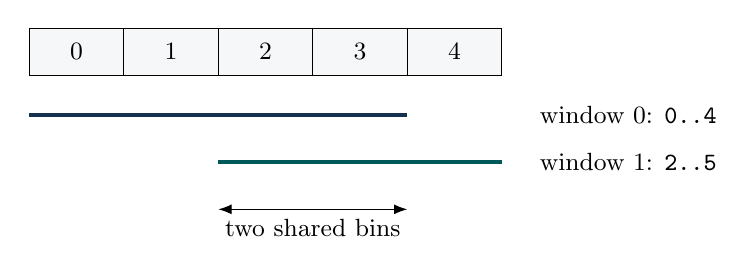
\begin{tikzpicture}[x=12mm,y=10mm,>=Latex]
\foreach \i in {0,...,4} {
  \draw[fill=ink!4] (\i,0) rectangle +(1,0.6);
  \node at (\i+0.5,0.3) {\small\i};
}
\draw[very thick,ink] (0,-0.5)--(4,-0.5);
\node[anchor=west,font=\small] at (5.3,-0.5) {window 0: \api{0..4}};
\draw[very thick,teal!70!black] (2,-1.1)--(5,-1.1);
\node[anchor=west,font=\small] at (5.3,-1.1) {window 1: \api{2..5}};
\draw[<->] (2,-1.7)--(4,-1.7);
\node[below,font=\small] at (3,-1.7) {two shared bins};
\end{tikzpicture}
\caption{An admissible two-window layout for the five levels of an eight-spin
periodic Ising chain.}
\end{figure}

Arrays retain the full global grid in each walker and mask bins outside its
window. For $R$ total walkers and $B$ global bins, histogram/DOS storage is
$O(RB)$, not the sum of local window lengths. The API has no automatic window
placement or memory-budget optimizer.

\section{Chunk execution and exchanges}
Rayon executes indexed walkers in bounded chunks. \api{exchange_every} is a
positive proposal interval. Seeds are assigned before parallel execution, so
successful seeded runs retain the documented reproducibility across Rayon thread
counts for the same implementation/platform and independent model behavior.
Worker panics become \api{WorkerFailed}; peer cancellation is checked between
proposals. A model callback still cannot be forcibly interrupted.

Alternating disjoint adjacent-window pairs attempt swaps between equal replica
indices. A trial is eligible only if both configurations fit the destination
supports. Following the window-exchange construction~\cite{moreno}, its log ratio
is
\begin{equation}
 r_{ij}=\ell_i(E_i)-\ell_i(E_j)+\ell_j(E_j)-\ell_j(E_i).
\end{equation}
State, parameter cache, energy, and current bin travel together. DOS, local RNG,
histograms, and adaptation schedules remain in their windows. An exchange does
not add a histogram visit or advance the SAMC clock.

A walker stops its adaptive chunk immediately when locally complete. If other
walkers remain active in later chunks, it makes frozen-DOS moves that increment
only \api{mixing_steps}. Once all walkers finish, no extra exchange is needed.
These counting rules are specific to this implementation and should be retained
when comparing with other replica-exchange WL codes.

\par\noindent\begin{minipage}{\linewidth}
% example: parallel_wl
\begin{lstlisting}[language=Rust,caption={Two overlapping windows with explicitly valid initial states.}]
use csta::wl::{run_parallel, Config, ParallelConfig, models::Ising};

fn main() -> Result<(), Box<dyn std::error::Error>> {
    let states = vec![
        Ising::<8>::new([1; 8])?,
        Ising::<8>::new([1, -1, 1, -1, 1, -1, 1, -1])?,
    ];
    let result = run_parallel(
        Ising::<8>::grid()?, states, (),
        ParallelConfig {
            windows: vec![0..4, 2..5],
            walkers_per_window: 1,
            exchange_every: 100,
            seed: 42,
            run: Config {
                preliminary_stages: 0,
                sampling_steps: 30_000,
                max_steps: 30_000,
                ..Config::default()
            },
        }, None,
    )?;
    let mut dos = result.merged.ok_or("no complete merged DOS")?;
    dos.normalize_log_count(256_f64.ln())?;
    println!("mean energy: {}", dos.energy_moments(0.5)?.0);
    Ok(())
}
\end{lstlisting}
\end{minipage}\par

\section{Averaging and joining DOS fragments}
After completion, replicas within a window are anchored to a common bin and
their log-DOS values are averaged. Each accessible level must have a lifetime
visit in every contributing replica. Adjacent window estimates are joined at
the overlap point minimizing their entropy-slope mismatch, aligned there, and
pasted. Endpoint slopes use secants; interior slopes use nonuniform three-point
derivatives. The construction follows the documented joining approach of
Moreno, Peralta, and Davis~\cite{moreno}.

Merged histograms sum actual current-stage counts from all contributing windows
and replicas, independent of the paste point. They do not count only the selected
DOS fragment. Missing visits, incompatible grids, or insufficient slope support
produce an error, rather than a fabricated merged spectrum.

\api{ParallelResult::merged} is present only if every walker reaches a nonzero
production target and joining succeeds. Cancellation and budget exhaustion
retain explicit partial walkers with no merged DOS; a worker or joining failure
returns an error. A successful merge establishes structural compatibility, not
small statistical error or absence of a join artifact.

\section{Parallel sessions and practical limits}
\api{ParallelSession<S,R>} exposes incremental \api{advance(chunks,cancel)} and
\api{finish}. Its unit is an exchange chunk, unlike serial session proposals.
Successful calls end at deterministic exchange barriers, suitable for exact
checkpoint continuation. A failed session is not reusable as a valid checkpoint.
Asynchronous cancellation can stop different walkers at different proposals;
resuming such a partial chunk need not reproduce an uninterrupted exchange
schedule.

This is shared-memory parallelism through Rayon. There is no MPI distribution,
GPU kernel, distributed checkpoint coordinator, or automatic load balancing of
energy-window difficulty. Replicas coupled by exchanges are not independent DOS
experiments for uncertainty estimation. Inspect coverage, exchange counts,
window disagreement, and independent complete runs.
\src{csta_wl/src/par_wl.rs}
\src{csta/examples/parallel_ising.rs}

\chapter{Observables, reweighting, and DOS uncertainty}\label{ch:analysis}
\section{Conditional observable moments}
An energy-only DOS does not determine an arbitrary observable. For $A(x)$,
\begin{equation}
 \mean{A}_\beta=\sum_i p_i(\beta)\mean{A\mid E\in I_i}.
\end{equation}
\api{analysis::ConditionalMoments} stores per-bin means of $A$ and $A^2$.
\api{record(energy,value)} validates the energy, value, and squared value and
updates atomically. \api{evaluate(dos,beta)} requires exactly compatible grids
and conditional observations on every finite-DOS bin, even if that bin's
canonical probability underflows at the requested temperature.

\api{Session::advance_observed} connects production states to this accumulator
without a new observer trait. It includes repeated retained states. Within-bin
samples must follow the intended conditional measure; adaptive transients and
poor mixing can bias them. Continuous-bin conditional reweighting additionally
approximates variation inside each interval.

\par\noindent\begin{minipage}{\linewidth}
% example: conditional
\begin{lstlisting}[language=Rust,caption={Recording an observable during a serial WL session.}]
use csta::wl::{Config, RawWangLandauData, Session, models::Ising};
use csta::wl::analysis::ConditionalMoments;
use rand::{SeedableRng, rngs::StdRng};

fn main() -> Result<(), Box<dyn std::error::Error>> {
    let grid = Ising::<4>::grid()?;
    let mut moments = ConditionalMoments::new(grid.clone());
    let mut session = Session::new(
        Ising::<4>::new([1; 4])?, (), StdRng::seed_from_u64(42),
        RawWangLandauData::on_grid(grid)?,
        Config { preliminary_stages: 0, sampling_steps: 20_000,
                 ..Config::default() },
    )?;
    session.advance_observed(20_000, None, |state, energy| {
        let m: f64 = state.spins().iter().map(|s| f64::from(*s)).sum();
        moments.record(energy, m)
    })?;
    let result = session.finish();
    if !result.is_complete() { return Err("partial run".into()); }
    let dos = result.data.process_data()?;
    println!("magnetization moments: {:?}", moments.evaluate(&dos, 0.5)?);
    Ok(())
}
\end{lstlisting}
\end{minipage}\par

\section{Single-histogram canonical reweighting}
\api{reweight(samples,source_beta,target_beta)} accepts pairs $(E_k,A_k)$ from a
stationary source canonical ensemble. It forms normalized weights
\begin{equation}
 w_k\propto e^{-(\beta_t-\beta_s)E_k},\qquad
 \widehat{\mean{A}}_t=\sum_k\widetilde w_k A_k,\qquad
 \ESS_w=\frac{1}{\sum_k\widetilde w_k^2}.
\end{equation}
An energy reference is subtracted and weights are normalized logarithmically.
Input must be nonempty and finite; unrepresentable log weights are errors.
At equal temperatures all weights are equal and the weighted mean is the ordinary
sample mean.

The result marks overlap as \api{Low} if $\ESS_w<20$ or $\ESS_w<0.1n$.
\api{Adequate} only means these thresholds passed. Weight ESS detects weight
concentration; it does not detect temporal correlation or states absent from the
source sample. It is not interchangeable with the autocorrelation ESS from
Chapter~\ref{ch:statistics}.

\par\noindent\begin{minipage}{\linewidth}
% example: reweight
\begin{lstlisting}[language=Rust,caption={Reweighting a nearby temperature from retained canonical samples.}]
use csta::{Metropolis, Schedule, models::Ising2D};
use csta::wl::analysis::reweight;
use rand::{SeedableRng, rngs::StdRng};

fn main() -> Result<(), Box<dyn std::error::Error>> {
    let mut run = Metropolis::with_all(
        Ising2D::aligned(4)?, (), 0.4, 12_000,
        StdRng::seed_from_u64(42),
    );
    let mut samples = Vec::new();
    run.run_observed(Schedule { burn_in: 2_000, stride: 1 }, None,
        |s, _| samples.push((s.recompute_energy(), s.magnetization())))?;
    let estimate = reweight(&samples, 0.4, 0.41)?;
    println!("{:?}", estimate);
    Ok(())
}
\end{lstlisting}
\end{minipage}\par

The helper changes temperature for a fixed effective Hamiltonian. It does not
implement WHAM, MBAR, automatic temperature-range selection, or general parameter
reweighting with missing sufficient observables. Joint DOS provides an explicit
field-dependent alternative in Chapter~\ref{ch:joint}.

\section{Independent DOS experiments}
\api{IndependentDos::from_run(id,result)} requires a complete run with nonzero
production. \api{from_data} allows external or exact data and assigns
responsibility for completion and independence to the caller. Unique IDs prevent
including the same labeled run twice; they cannot establish statistical
independence or detect duplicated data under different IDs.

\api{DosEnsemble::new(runs,log_count)} requires matching grids and finite-support
patterns and normalizes each run to the same total count. It evaluates an
observable on each normalized DOS, then returns its mean and
$\SE=\sqrt{s^2/R}$ across $R$ runs. One run has no standard error.
\api{log_dos_uncertainty} reports per-bin disagreement, with absent bins left
undefined. This preserves nonlinear observable evaluation per experiment rather
than treating all walkers as independent observations of one averaged DOS.

\par\noindent\begin{minipage}{\linewidth}
% example: dos_ensemble
\begin{lstlisting}[language=Rust,caption={Uncertainty across separately seeded DOS experiments.}]
use csta::wl::{self, Config, RawWangLandauData, models::Ising};
use csta::wl::analysis::{DosEnsemble, IndependentDos};
use rand::{SeedableRng, rngs::StdRng};

fn main() -> Result<(), Box<dyn std::error::Error>> {
    let mut runs = Vec::new();
    for id in 0..3 {
        let result = wl::run(
            Ising::<4>::new([1; 4])?, (),
            StdRng::seed_from_u64(42 + id),
            RawWangLandauData::on_grid(Ising::<4>::grid()?)?,
            Config { preliminary_stages: 0, sampling_steps: 10_000,
                     ..Config::default() }, None,
        )?;
        runs.push(IndependentDos::from_run(id, result)?);
    }
    let ensemble = DosEnsemble::new(runs, 16_f64.ln())?;
    println!("{:?}", ensemble.energy(0.5)?);
    Ok(())
}
\end{lstlisting}
\end{minipage}\par

Between-run scatter does not include a bias shared by every run, an incorrect
support declaration, or finite-bin quadrature error. There is no automatic
independence test, confidence-interval calibration, or convergence certificate.
\src{csta_wl/src/analysis.rs}

\chapter{Sparse joint density of states}\label{ch:joint}
\section{Coordinates and field reweighting}
\api{joint::JointGrid} declares a sparse list of accessible $(E_0,M)$ cells,
where $E_0$ excludes an external magnetic field. Cells must be finite, unique,
lexicographically sorted, nonempty, and no more numerous than the supplied
\api{max_cells}. This checks the declared cell count; a caller can already have
allocated an oversized vector before invoking the constructor.

\api{JointDos} requires one finite log mass on each declared cell. Missing cells
are outside support, not entries inferred from a zero histogram. For finite
$\beta,h$, evaluation uses
\begin{equation}
 Z(\beta,h)=\sum_{E_0,M}g(E_0,M)
       e^{-\beta(E_0-hM)}.
\end{equation}
It returns log partition function, mean physical energy $E_0-hM$, total
magnetization, and cell probabilities. Normalization fixes the total state count.
\api{energy_marginal} sums over $M$ with log-sum-exp and produces an energy DOS
in $E_0$, appropriate to the zero-field projection.

\par\noindent\begin{minipage}{\linewidth}
% example: joint
\begin{lstlisting}[language=Rust,caption={An exact one-spin joint spectrum and field response.}]
use csta::wl::joint::{JointDos, JointGrid};

fn main() -> Result<(), Box<dyn std::error::Error>> {
    let grid = JointGrid::new(vec![(0.0, -1.0), (0.0, 1.0)], 2)?;
    let dos = JointDos::new(grid, vec![0.0, 0.0])?;
    let beta = 0.5;
    let field = 0.3;
    let thermal = dos.evaluate(beta, field)?;
    assert!((thermal.magnetization - (beta * field).tanh()).abs()
        < 1e-14);
    assert!((thermal.energy + field * thermal.magnetization).abs()
        < 1e-14);
    assert_eq!(dos.energy_marginal()?.grid().len(), 1);
    Ok(())
}
\end{lstlisting}
\end{minipage}\par

\section{Joint sampling through the existing engine}
\api{run_joint} takes a \api{State}, parameters, RNG, declared cells, a read-only
magnetization closure, ordinary WL configuration, and optional cancellation.
The state's energy must be $E_0$. An adapter maps each exact $(E_0,M)$ cell to an
index represented as a discrete pseudo-energy; the existing WL engine then
flattens those cells. Finite undeclared cells are rejected; nonfinite coordinates
are errors. The proposal-ratio hook is forwarded.

The adapter evaluates the underlying energy instead of forwarding its optional
local-energy shortcut. Its cell search costs $O(\log K)$ for $K$ declared cells,
and DOS storage is $O(K)$. A large state space can remain impractical even when
sparse. No automatic reachability discovery, adaptive cell insertion, continuous
multidimensional interpolation, or generalized collective-variable framework is
implemented.

The returned \api{JointRun} contains original state, parameters, joint DOS, and
WL diagnostics, with the same explicit completion rule. It does not expose a
full per-cell histogram API or a dedicated serializable joint session. Field
responses beyond the returned means can be computed from cell probabilities,
but joint heat-capacity and susceptibility convenience methods are not supplied.

\par\noindent\begin{minipage}{\linewidth}
% example: joint_sampling
\begin{lstlisting}[language=Rust,caption={Sampling explicitly enumerated joint support for a three-spin chain.}]
use csta::State;
use csta::wl::{Config, models::Ising};
use csta::wl::joint::{JointGrid, run_joint};
use rand::{SeedableRng, rngs::StdRng};

fn magnetization(s: &Ising<3>) -> f64 {
    s.spins().iter().map(|x| f64::from(*x)).sum()
}

fn main() -> Result<(), Box<dyn std::error::Error>> {
    let mut cells = Vec::new();
    for bits in 0..8 {
        let spins = std::array::from_fn(|i| {
            if bits & (1 << i) == 0 { -1 } else { 1 }
        });
        let state = Ising::<3>::new(spins)?;
        cells.push((state.energy(&mut ()), magnetization(&state)));
    }
    cells.sort_by(|a, b| a.partial_cmp(b).unwrap());
    cells.dedup();
    let mut result = run_joint(
        Ising::<3>::new([1; 3])?, (), StdRng::seed_from_u64(42),
        JointGrid::new(cells, 8)?, magnetization,
        Config { preliminary_stages: 0, sampling_steps: 20_000,
                 ..Config::default() }, None,
    )?;
    if !result.is_complete() { return Err("partial joint run".into()); }
    result.data.normalize_log_count(8_f64.ln())?;
    println!("{:?}", result.data.evaluate(0.5, 0.2)?);
    Ok(())
}
\end{lstlisting}
\end{minipage}\par

Enumeration here establishes support independently of sampling; it is practical
only for this tiny system. For a larger model, derive accessible cells from its
constraints or another validated support construction.
\src{csta_wl/src/joint.rs}

\chapter{Persistence and reproducible continuation}\label{ch:checkpoint}
\section{Opt-in serialization}
Enable \api{checkpoint} for sampler save/load methods. Supported types are
\api{Metropolis}, serial and parallel WL sessions, and temperature replica exchange.
State, parameters, and RNG must implement the required Serde traits; parameters
must still clone independently. Built-in lattice and WL reference models provide
feature-gated support, subject to Serde support for their concrete array sizes.

\api{CheckpointRng} is PCG64 from pinned \api{rand_pcg} 0.10.2. Use it when a
serializable random stream is required. The default \api{StdRng} is not supported
by these serialization bounds. For temperature exchange, use
\api{ReplicaExchange::<_, CheckpointRng>::seeded}; for parallel WL, choose the RNG
type on \api{ParallelSession}. Merely enabling the feature does not make every
RNG serializable.

\par\noindent\begin{minipage}{\linewidth}
% example: checkpoint
\begin{lstlisting}[language=Rust,caption={Saving and continuing a canonical run; requires the checkpoint feature.}]
use csta::{CheckpointRng, Metropolis, models::Ising2D};
use rand::SeedableRng;

fn main() -> Result<(), Box<dyn std::error::Error + Send + Sync>> {
    let path = std::env::temp_dir().join(format!(
        "csta-design-{}.json", std::process::id()));
    let mut run = Metropolis::with_all(
        Ising2D::aligned(4)?, (), 0.4, 100,
        CheckpointRng::seed_from_u64(42),
    );
    run.run(None)?;
    run.save(&path, "ising-j1-h0-v1")?;
    let mut resumed = Metropolis::<Ising2D, CheckpointRng>::load(
        &path, "ising-j1-h0-v1",
    )?;
    resumed.run(None)?;
    assert_eq!(resumed.attempted_moves, 200);
    std::fs::remove_file(path)?;
    Ok(())
}
\end{lstlisting}
\end{minipage}\par

\section{File format and validation}
The generic core envelope stores format version 1, an implementation tag,
caller model tag, Rust type name, and serialized value. The implementation tag is
\path{csta-3/checkpoint-1/rand-0.10.2}. Model tags must be nonempty on save and should change with a
Hamiltonian or model schema change. Type names and tags detect mismatches; they
do not independently prove physical compatibility.

Saving serializes the value to JSON in memory, creates a sibling temporary file,
writes and synchronizes it, renames it to the destination, and synchronizes the
parent directory. Temporary-name collisions are retried with a bounded count.
Pre-save validation and serialization failures leave an existing destination
untouched. A filesystem error after rename can be reported even though the
replacement already occurred; the operation is not a multi-file transaction.

Loading reads at most 256 MiB plus one byte to detect an oversized file. It checks
envelope compatibility and then sampler-specific invariants: grid shape,
support, counters, phase/schedule consistency, and cached state energy.
\api{State::valid_state} supplements energy checks for structural constraints.
The low-level generic core loader does not itself know a model's physical
invariants. DOS values use floating bit patterns to preserve negative infinity
and finite values exactly; JSON float round-trip support preserves other stored
floating values.

Files are intended as trusted local snapshots. There is no cryptographic
integrity check, signature, compression, cross-version migration, or arbitrary
schema conversion. The input-byte limit is not a general cap on all allocations
made during deserialization. Large simulations may exceed the current persistence
format's practical range.

\section{What continuation preserves}
Serial WL snapshots retain state, parameter cache, RNG, grid, DOS, both
histograms, bin/energy cache, preliminary stage, SAMC clock, target, and total
budget. Parallel snapshots also retain exchange RNG, parity, and window state at
successful barriers. Temperature replicas retain labels and pending local-chunk
position. Canonical snapshots retain configured per-call steps and lifetime
counters; the next \api{run} starts another configured budget, not an inferred
remainder of a previous call.

External observation vectors, file cursors, closures, and application-level
analysis are not automatically saved. Coordinating their state with the sampler
is required to avoid duplicated or missing measurements after a restart.
Measurement schedules that restart per call also need deliberate handling by
the application.

Exact continuation is scoped to the same implementation, dependencies, platform,
and deterministic model/callback behavior. Restoring a saved RNG cannot undo
nondeterministic external input or shared mutable aliases. Successful parallel
barriers provide a stronger reproducibility boundary than asynchronous mid-chunk
cancellation. A previous DOS plus fresh counters is a new run, regardless of
whether its initial numerical values match a snapshot.
\src{csta_core/src/checkpoint.rs}
\src{csta_montecarlo/src/lib.rs}
\src{csta_wl/src/session.rs}
\src{csta_wl/src/par_wl.rs}
\src{csta_metropolis/src/replica.rs}

\chapter{Validation, cost, and design boundaries}\label{ch:validation}
\section{Error and partial-result policy}
\begin{longtable}{@{}P{0.27\textwidth}P{0.67\textwidth}@{}}
\toprule Interface & Failure meaning and boundary\\\midrule\endhead
Vector arithmetic & IEEE results; checked direction is \api{Option}, not a
universal checked-math layer.\\
Geometry/dynamics & Static-string errors for invalid dimensions, nonfinite
coordinates, invalid forces, or numerical failures. One dynamics step commits
only after validation.\\
Random construction & \api{Randomizable} is infallible. Dynamic invalid ranges,
invalid const-generic reference-model sizes, and allocation failures can panic.\\
Canonical checked API & \api{Error(&'static str)}; proposal errors restore state,
parameters, and counters under the model contract. RNG is not rewound.\\
Canonical legacy API & Convenience execution can panic. Use \api{try_step} or
checked run methods when errors must be handled.\\
Streaming callback & Failure occurs after the observed move commits; external
side effects are not transactional.\\
Statistics & Invalid/numerically unrepresentable observations give errors;
short, constant, or unresolved uncertainty data can give \api{None}.\\
Serial WL & Typed invalid-input, energy, support, counter, and numerical errors;
cancellation/budget stops return explicit partial results.\\
Parallel WL & Worker panic or joining failure is an error. Partial sampling has
no apparently successful merged DOS. Model hangs cannot be preempted.\\
Checkpoint & Boxed I/O, format, or validation errors; model tag and structural
validation remain necessary.\\
\bottomrule
\end{longtable}

\section{Operation and memory costs}
Let $N_s$ be lattice sites, $N_p$ particles, $D$ dimension, $B$ energy bins,
$R$ total WL walkers, $n$ observations, and $C_P$ the cost of cloning parameters.
The table describes the implementation, excluding user callback cost unless
stated. These are operation counts, not measured throughput claims.

\begin{longtable}{@{}P{0.30\textwidth}P{0.31\textwidth}P{0.32\textwidth}@{}}
\toprule Operation & Work & Additional storage\\\midrule\endhead
Small vectors & Constant dimension & Constant\\
Periodic wrap/displacement & $O(D)$ & $O(D)$ output\\
Ising local proposal & $O(1)+C_P$ with cached energy & Change plus parameter snapshot\\
Wolff update & $O(N_s)$ including energy recomputation & $O(N_s)$ scratch\\
Moment/block update & $O(1)$ & $O(1)$\\
Correlation estimate & $O(n\min(n/2,4096))$ & Retained $O(n)$ input\\
Thermal jackknife & $O(n+B_k^2)$, $B_k$ blocks & $O(B_k)$ summaries plus input\\
Block bootstrap & $O(R_b n)$ plus statistic cost & $O(n)$ resampled series\\
Harmonic dynamics step & $O(N_pD)$ & $O(N_pD)$ candidate/forces\\
Lennard--Jones step & $O(N_p^2D)$ & $O(N_pD)$ candidate/forces\\
Serial WL proposal & Model work, $C_P$, lookup, update & $O(B)$ retained arrays\\
Preliminary flatness test & $O(B)$ when minimum visits reached & Constant beyond arrays\\
Parallel WL storage & Per-walker computation and barriers & $O(RB)$ plus states/caches\\
DOS thermal evaluation & $O(B)$ & $O(B)$ weights/output\\
Sparse joint lookup & $O(\log K)$ for $K$ cells & $O(K)$ DOS/support\\
Checkpoint save/load & Linear in serialized size & Full JSON buffer and decoded state\\
\bottomrule
\end{longtable}

Energy-grid lookup uses ordered searches; continuous grids retain edges rather
than silently relying on a rounding-sensitive arithmetic index. Preliminary
flatness scans can dominate cheap models after the visit minimum. Parameter
cloning is part of every checked proposal; a large cache can erase the benefit
of a local energy difference. Profile the actual model before adding complexity.
Neither checked sizes nor finite budgets guarantee that arbitrary allocations
will fit available memory.

\section{Existing verification strategy}
\path{TEST_PLAN.md} maps the workspace's test groups, including ordinary and edge
cases. The current suite combines deterministic unit tests, facade integration,
compile-fail macro examples, seeded bounded simulations, exact small-spectrum
checks, and an explicitly ignored longer release test. This document does not
replace that coverage map or claim every possible physical regime is tested.

\begin{longtable}{@{}P{0.24\textwidth}P{0.70\textwidth}@{}}
\toprule Area & Important average and boundary checks\\\midrule\endhead
Vectors/geometry & Coordinate-preserving casts, arithmetic agreement, tiny/huge
normalization, zero/nonfinite directions, periodic endpoints and half-box ties,
unique bonds and invalid dimensions.\\
Random/derive & Seed repeatability, range bounds, vector/enum construction,
zero weights, invalid syntax, dependency cycles, distribution moments and sphere
isotropy with explicit tolerances.\\
Canonical/models & Exact apply/revert including caches, retained-state counting,
observer timing, cancellation, asymmetric proposals, nonfinite energies,
zero attempts, Ising local differences, gas energy conventions, cluster limits.\\
Statistics & Known moments, merge agreement, missing/constant data, complete
block handling, correlated synthetic series, nonlinear errors, ambiguous curve
crossings and boundary peaks.\\
Dynamics & Harmonic trajectory and step-size scaling, force finite differences,
momentum conservation, invalid masses/time steps, coincident pairs, failed-step
rollback.\\
Serial WL & Exact energy mapping, masks, one visit per completed trial,
preliminary/production clocks, finite off-support rejection, numerical failure,
zero target, cancellation, and total-budget exhaustion.\\
DOS analysis & Exact finite spectra, stable shifted weights, normalization,
absent levels, negative/zero beta, conditional support, weight overlap, duplicate
independent-run IDs, and joint-field response.\\
Parallel/checkpoint & Window validation, exchange counts, frozen mixing,
thread-count reproducibility, incomplete merge rejection, worker errors,
continuous versus resumed trajectories, invalid formats/tags/caches, and file
replacement behavior.\\
\bottomrule
\end{longtable}

Run repository checks with the required toolchain:
\par\noindent\begin{minipage}{\linewidth}
\begin{lstlisting}[caption={Workspace validation from the repository root.}]
cargo fmt --all -- --check
cargo check --workspace --all-targets --all-features
cargo test --workspace
cargo test --workspace --all-features
cargo clippy --workspace --all-targets --all-features -- -D warnings
cargo test -p csta_wl --release -- --ignored
\end{lstlisting}
\end{minipage}\par
The final command is a deliberate longer stochastic check. Use fixed seeds,
finite budgets, exact references where practical, and explicit tolerances.
Repeated success of a finite simulation is not proof of universal convergence.
Documentation examples are checked separately against the local facade so that
API drift is caught without treating demonstration output as a scientific result.

\section{Scientific validation beyond API correctness}
For canonical simulations, compare independent initial states and seeds, inspect
observables with different relaxation scales, vary burn-in and block lengths,
and verify exact small-system averages. Check signed and absolute order
parameters deliberately. A low error estimate on a trapped trajectory is not a
reliable physical uncertainty.

For DOS simulations, validate accessible support and proposal connectivity,
compare independently normalized DOS estimates, inspect lifetime coverage and
window overlaps, vary preliminary/production budgets, and repeat with narrower
continuous bins or wider cutoffs. Compare thermodynamics over the intended
$\beta$ range, where rare levels can receive large canonical weight.

For dynamics, compare numerical forces with potential derivatives, test the
conserved quantities appropriate to the force law, halve the time step, and
check trajectory and drift sensitivity. Potential correctness and integrator
correctness are separate. A stable finite time series does not establish bulk
transport properties or a thermodynamic limit.

\section{Deliberate boundaries and extension rules}
The implemented range remains explicit. There is no general tensor algebra,
arbitrary graph lattice, triclinic geometry, automatic equilibration detector,
universal proposal distribution, WHAM/MBAR solver, critical-exponent fitter,
production molecular-dynamics force engine, MPI/GPU backend, or cross-version
checkpoint migration. Higher-dimensional joint support and rare-event methods
require model-specific choices that the current API does not guess.

An extension should keep the common workflow small. Add it to the owning crate,
retain the facade dependency direction, give new hooks defaults where possible,
and prefer an explicit module or wrapper to new mandatory model methods.
Preserve independent parameter rollback and retained-proposal counting. New
samplers need finite execution controls and explicit partial results. New
numerics need units, valid input ranges, undefined-output behavior, and reference
cases before performance claims.

A proposed optimization must preserve seeded behavior where that behavior is
part of the documented contract, or document the change. A new physical model
must state its ensemble, boundary convention, proposal symmetry, cache invariant,
and energy normalization. Optional capability should not impose additional
configuration on existing basic runs.
\src{AGENTS.md}
\src{TEST_PLAN.md}
\src{TODO.md}

\appendix
\chapter{Source and example map}\label{app:source}
\section{Owning implementation files}
\begin{longtable}{@{}P{0.54\textwidth}P{0.40\textwidth}@{}}
\toprule Path & Role\\\midrule\endhead
\path{csta/src/lib.rs}, \path{csta/src/prelude.rs} & Facade exports and observer prelude.\\
\path{csta_core/src/lib.rs} & Core module declarations.\\
\path{csta_core/src/vec2.rs}, \path{csta_core/src/vec3.rs}, \path{csta_core/src/vec4.rs} & Vector types and operators.\\
\path{csta_core/src/geometry.rs} & Periodic boxes and lattice bonds.\\
\path{csta_core/src/dynamics.rs} & NVE state, Verlet, force helpers.\\
\path{csta_core/src/checkpoint.rs} & Feature-gated JSON envelope and atomic replacement.\\
\path{csta_montecarlo/src/lib.rs} & Random trait, iterator, distributions, PCG alias.\\
\path{csta_derive/src/lib.rs} & Macro parsing, dependencies, code generation.\\
\path{csta_metropolis/src/lib.rs} & State and canonical runner.\\
\path{csta_metropolis/src/observer.rs} & Static and dynamic observer contracts.\\
\path{csta_metropolis/src/models.rs} & Ising2D, lattice gas, Wolff.\\
\path{csta_metropolis/src/statistics.rs} & Streaming and correlated statistics.\\
\path{csta_metropolis/src/finite_size.rs} & Curves and block bootstrap.\\
\path{csta_metropolis/src/replica.rs} & Temperature exchange and persistence.\\
\path{csta_wl/src/grid.rs} & Energy support and lookup.\\
\path{csta_wl/src/lib.rs} & Raw data, configuration, walker, run APIs.\\
\path{csta_wl/src/wl_data.rs} & DOS normalization and thermodynamics.\\
\path{csta_wl/src/models.rs} & 1D Ising and quantum oscillators.\\
\path{csta_wl/src/par_wl.rs} & Rayon chunks, exchange, joining, parallel session.\\
\path{csta_wl/src/session.rs} & Serial continuation and walker snapshot checks.\\
\path{csta_wl/src/analysis.rs} & Conditional moments, reweighting, independent DOS.\\
\path{csta_wl/src/joint.rs} & Sparse joint support and field reweighting.\\
\path{csta_wl/src/main.rs} & Ising/oscillator DOS demonstration binary.\\
\bottomrule
\end{longtable}

\section{Runnable repository examples}
Run these from the workspace root. Simulation durations and output volumes vary.
The document's shorter embedded examples are independent of these programs.
\par\noindent\begin{minipage}{\linewidth}
\begin{lstlisting}[caption={Repository examples and demonstration binaries.}]
cargo run -p csta --release --example state
cargo run -p csta --release --example rand_derive
cargo run -p csta --release --example ising
cargo run -p csta --release --example physics
cargo run -p csta --release --example hastings
cargo run -p csta --release --example reweight
cargo run -p csta --release --example finite_size
cargo run -p csta --features checkpoint --example checkpoint
cargo run -p csta --release --example parallel_ising
cargo run -p csta --release --example profile_energy
cargo run -p csta_wl --release
cargo run -p csta_wl --release -- qho
\end{lstlisting}
\end{minipage}\par
\path{state.rs} demonstrates a custom model; \path{rand_derive.rs} demonstrates
random construction. \path{physics.rs} combines selected physics tools.
\path{finite_size.rs} emits size/temperature observables and uncertainties.
\path{profile_energy.rs} compares energy-evaluation paths; its timings depend on
build profile and hardware. The default WL binary uses an Ising chain; the
\api{qho} argument chooses the truncated oscillator example.

\chapter{Example and document reproducibility}
The standalone programs in this document are marked by \api{example:} comments
in the TeX source. \path{docs/check_examples.py} extracts only those listings,
creates a temporary Cargo package depending on the local facade, and checks or
runs them. The checkpoint program is validated with its feature enabled. Trait,
manifest, and command excerpts are intentionally excluded from extraction.

\par\noindent\begin{minipage}{\linewidth}
\begin{lstlisting}[caption={Build and validate the document from the workspace root.}]
latexmk -pdf -interaction=nonstopmode -halt-on-error \
  -outdir=docs/build docs/design.tex
python3 docs/check_examples.py --offline
python3 docs/check_examples.py --offline --run
\end{lstlisting}
\end{minipage}\par
\api{--offline} is appropriate only when dependencies are already cached. The
checker uses temporary sources and a build cache under \path{target/}; it does
not add a workspace member or change the library API. The PDF needs standard
LaTeX packages listed in the source preamble. Build byproducts are kept in the
ignored \path{docs/build/} directory. The distributed PDF is
\path{docs/design.pdf}; copy the rebuilt PDF there when updating it.

Embedded assertions check exact API invariants or small analytic values.
Simulation examples check finite execution and explicit result handling, not a
general convergence tolerance. Their printed values are intentionally not
included as published physical measurements.

\begin{thebibliography}{9}
\addcontentsline{toc}{chapter}{References}
\bibitem{moreno}
F. Moreno, J. Peralta, and S. Davis.
\emph{A portable and flexible implementation of the Wang--Landau algorithm in
order to determine the Density of States}. arXiv:2103.15028v2 (2021).
\url{https://arxiv.org/abs/2103.15028v2}.
Referenced for window exchange and slope-based joining; CSTA's counters and
SAMC composition are specified by its own implementation.

\bibitem{shakirov}
T. Shakirov. \emph{Flat-histogram algorithms: optimal parameters and extended
application}. arXiv:2402.05653v2 (2024).
\url{https://arxiv.org/abs/2402.05653v2}.
Referenced for the trial-move SAMC schedule. CSTA does not implement every
extension described in the paper.

\bibitem{geyer}
C. J. Geyer. \emph{Initial Sequence Estimators}, documentation for the
\api{mcmc} package, referring to \emph{Practical Markov Chain Monte Carlo},
Statistical Science 7, 473--483 (1992).
\url{https://www.stat.umn.edu/geyer/mcmc/library/mcmc/html/initseq.html}.
CSTA uses monotone positive pairs, a finite lag cap, and a conservative time floor.

\bibitem{janke}
W. Janke. \emph{Monte Carlo Simulations in Statistical Physics---From Basic
Principles to Advanced Applications}. Lecture chapter (2012).
\url{https://www.physik.uni-leipzig.de/~janke/Paper/lviv-ising-lecture-janke_corrected.pdf}.
Referenced for the ferromagnetic cluster construction.

\bibitem{lammps}
LAMMPS developers. \emph{fix nve command}, LAMMPS documentation.
\url{https://docs.lammps.org/fix_nve.html}.
Referenced for the velocity-Verlet integration method. CSTA does not wrap LAMMPS
or provide its force-field infrastructure.

\end{thebibliography}
\end{document}
